% ------% % Uncomment and use as if needed
% \newtheorem{theorem}{Theorem}
% \newtheorem{lemma}[theorem]{Lemma}
% \newtheorem{proposition}[theorem]{Proposition}
% \newtheorem{definition}[theorem]{Definition}
% \newdefinition{remark}{Remark}
% \newtheorem{corollary}[theorem]{Corollary}

% %----------------New Commands---------------%
% \newcommand{\innerprod}[1]{\left\langle #1 \right\rangle}
% \newcommand{\abs}[1]{\lvert #1 \rvert}
% \newcommand{\bigabs}[1]{\left \lvert #1 \right \rvert}

% \newcommand{\sobkp}[1]{W^{k,p}(#1)}
% \newcommand{\sob}{W^{k,p}}
% \newcommand{\Lloc}[1]{L_1^{loc}(#1)}
% \newcommand{\totalV}[1]{D_t^{\abs{#1}}V(t)}
% \newcommand{\totalJ}[1]{D_t^{\abs{#1}}J(t)}
% \newcommand{\D}{\textbf{D}}
% \newcommand{\fhat}{\hat{f}}

% %minGW
% \newcommand{\argminpsi}{\min\limits_{g(\textbf{w}(t),\psi(t))\in \sob}}

% %minSmoothGW
% \newcommand{\minSmoothGW}{\min\limits_{g(\textbf{w}(t),\delta(\psi(t)))\in \sob}}


% \let\WriteBookmarks\relax
% \def\floatpagepagefraction{1}
% \def\textpagefraction{.001}

% % Short title
% \shorttitle{}    

% % Short author
% \shortauthors{}  

% % Main title of the paper
% \title [mode = title]{The Effect of Architechture on Learning Behavior of Deep Neural Networks}  

% % Title footnote mark
% % eg: \tnotemark[1]
% %\tnotemark[1] 

% % Title footnote 1.
% % eg: \tnotetext[1]{Title footnote text}
% \tnotetext[1]{} 

% % First author
% %
% % Options: Use if required
% % eg: \author[1,3]{Author Name}[type=editor,
% %       style=chinese,
% %       auid=000,
% %       bioid=1,
% %       prefix=Sir,
% %       orcid=0000-0000-0000-0000,
% %       facebook=<facebook id>,
% %       twitter=<twitter id>,
% %       linkedin=<linkedin id>,
% %       gplus=<gplus id>]

% \author[1]{Allyson Hahn}%[<options>]]

% % Corresponding author indication
% \cormark[1]

% % Footnote of the first author
% \fnmark[1]

% % Email id of the first author
% \ead{}

% % URL of the first author
% \ead[url]{}

% % Credit authorship
% % eg: \credit{Conceptualization of this study, Methodology, Software}
% \credit{}

% % Address/affiliation
% \affiliation[1]{organization={Department of Mathematical Sciences, Northern Illinois University}}

% \author[2]{Krishnan Raghavan}%[]

% % Footnote of the second author
% \fnmark[2]

% % Email id of the second author
% \ead{}

% % URL of the second author
% \ead[url]{}

% % Credit authorship
% \credit{}

% % Address/affiliation
% \affiliation[2]{organization={Mathematics and Computer Science Division, Argonne National Laboratory}}

% % Footnote text
% \fntext[1]{}

% % For a title note without a number/mark
% %\nonumnote{}

% %-------------------Abstract-----------------------%
% \begin{abstract}
% We consider the effects of Neural Network architecture in the setting of continual learning. Using dynamic programming we complete a bilevel optimization to determine the optimal architecture for the current and previous task data followed by the optimal weights for the network. 
% \end{abstract}

% % Use if graphical abstract is present
% %\begin{graphicalabstract}
% %\includegraphics{}
% %\end{graphicalabstract}

% %-----------------Highlights------------------%
% \begin{highlights}
% \item The first quantification of NN architecture on the learning behavior
% \item Demonstrate the conditions to ensure stability of neural networks.
% \item A novel measure to efficiently perform neural architecture search and hyper-parameter search.
% \end{highlights}
% %-------------------Keywords-------------------%
% \begin{keywords}
%  Neural Network \sep Architecture Search\sep  \sep
% \end{keywords}
% \maketitle
\section{Introduction}
With the advent of large-scale AI models, the computational expense of training such models has also increased drastically; training these models efficiently often requires large-scale high-performance computing infrastructure. Despite such drastic expenditure, these models quickly become stale. The reason  is that the data distribution shifts or new data  gets generated, 
%as these models often drift~(become stale)
%due to change in the data distribution
requiring realignment. This necessity presents a quandary. Naive realignment leads to a phenomenon called catastrophic forgetting, where the model overwrites prior information. On the other hand, a complete retraining of the model would require significant resources, a solution that is extremely unattractive. 

A more viable option is  continual learning, where approaches seek to constrain the parameters of the model to reduce the amount of catastrophic forgetting the model experiences. Several works in the literature have attempted this direction, starting from early work on small multilayer perceptrons~\cite{mccloskey1989catastrophic} to recent works on large language models such as \cite{luo2025empirical, lai2025reinforcement, biderman2024lora} and \cite{lin2025continual}. One key commonality across all  these approaches is that they look to constrain the weight/parameters of the AI model to induce minimal forgetting. On the other hand, and more appropriately, some approaches seek a balance between forgetting and the learning of new data~(generalization); see, for example, ~\cite{raghavan2021formalizing, lu2025rethinking,lin2023theory}. Despite demonstrated success, this is not the full story. In fact,  under mild assumptions, it has been proven that simply changing the weight of the AI model is not sufficient to capture the drift in the data distribution, and the capacity of the neural network (its ability to represent tasks) eventually diverges if the data distribution keeps changing ~\cite{chakraborty2025understanding}. These intractability results from \cite{chakraborty2025understanding} highlight a conundrum:  if the capacity of the network eventually diverges, then should we still aim to continually train AI models?
%even though continually learning such models is invaluable? 
In this paper we demonstrate that the answer to this question is indeed ``yes"; in fact, \textit{the solution is to reliably change the architecture of the AI model on the fly according to the needs of the data distribution.} 

However,  three key bottlenecks remain before attaining this goal. (i) Reliably changing the architecture requires a methodical understanding of ``how the weights and the architecture of the model interact with each other," that is, the coupling between the weights and the architecture. (ii) Moreover, to decide when to change the architecture, one must understand how the forgetting-generalization trade-off is affected by the aforementioned coupling. Loosely speaking, the first two bottlenecks have been heuristically addressed in the literature. For example, some recent works such as  CLEAS (Continual Learning with Efficient Architecture Search)~\cite{CLEASgao2022CLEAS} and SEAL (Searching Expandable Architectures for Incremental Learning)~\cite{SEALgambella2025SEAL} involve dynamically expanding the capacity of the AI model by adding layers and defining metrics that govern the necessity for a change in capacity. However, none of these approaches involves or enables a generic ability to change different aspects of the architecture, number of parameters, activation functions, layers, and so forth. The key reason is that if the architecture is generically changed, one must initialize the new network architecture at random. (iii) Then, the transfer of information about the weights from the previous architecture to the new architecture across parameter spaces of two different shapes is required. Doing so, however,  is currently impossible. In the absence of such a transfer mechanism, current approaches such as CLEAS and SEAL can  modify only those components that would not warrant information transfer between parameter space of two different sizes. 

To address these bottlenecks, we  present a comprehensive approach that includes a new formulation to understand the coupling between the architecture and the weights of the model, a methodical way of searching for a generic new architecture, and a novel method for transferring information between the old  and the new architecture.


\subsection{Contribution}
The key reason the coupling between the architecture and the weights is difficult to model is that architecture dependencies are observed on a function space across tasks and the weight dependencies are visible across the Euclidean parameter space. Any modeling in the weight space such as presented in \cite{chakraborty2025understanding, raghavan2021formalizing} or \cite{lu2025rethinking} cannot capture function space dependencies. To obviate this situation, we model the problem of continually training the AI model over a sequence of tasks in a Sobolev space. Using this theoretical framework, we describe how, in the Sobolev space of AI models parameterized by architecture choices and  weights, weights alone cannot capture the change in the distribution:  the architecture must be changed. We then employ a derivative-free architecture search  to determine the new architecture by searching for an appropriate number of neurons.  Although we focus on changing the number of parameters in the AI model, our work is general enough to extend to other architecture choices as well. Once the new architecture is chosen, we develop a new algorithm that can efficiently transfer information from the previous architecture to a new architecture across parameter spaces of different sizes with minimal loss of performance on the previous tasks.

We  empirically demonstrate that changing the architecture indeed results in better training loss compared with when the architecture is not changed. We also show that our algorithm achieves substantial improvements in terms of training loss when training over large numbers of tasks; it is robust to noise and scales from feedforward neural networks to graph neural networks seamlessly across regression and classification problems. We envision that jointly training the architecture and the weights in the continual learning paradigm is the best path forward in the field of continual learning, and we develop the basic theoretical and empirical infrastructure to allow for such training. 


\subsection{Organization}
The paper is organized as follows. We begin with a description of continual learning (CL) and motivate the necessity for function space modeling. Next, we describe a collection of neural networks as functions in a Sobolev space. We then derive the necessary condition for the existence of a CL solution and demonstrate that weights alone are not enough to train a network efficiently. Thus, we describe the need to change the architecture of the network along with the weights of the AI model. We  present an algorithm to change the architecture on the fly and transfer information between the two architectures. We describe empirically the advantages of our approach and conclude with a brief summary. 


\subsection{Notation}
The notation is adapted from \cite{kolda2009tensor}; please refer to the original paper for additional details. We use $\mathbb{N}$ to denote the set of natural numbers and $\mathbb{R}$ to denote the set of real numbers.  An $m^{th}$-order tensor is viewed as a multidimensional array contained in $\mathbb{R}^{I_1 \times I_2 \times I_3 \times I_4 \times \cdots I_{m}}$,  where the order can be thought of as the number of dimensions in the tensor. In this paper we will  be concerned mostly with tensors of order $0, 1, 2$ and $3$, which correspond to scalars, vectors, matrices, and a list of matrices. Therefore, we will write a tensor of order $0$ as a scalar with lowercase letters,  $\sx;$  a tensor of order one is denoted by lowercase bold letters such as $\vx.$ A tensor of order $2$ is 
denoted by uppercase bold letters $\mx$, and any tensor of order greater than $2$ is denoted by bolder Euler scripts letters such as $\tx.$  We also use $\|.\|$ to denote the Euclidean norm for vectors, Frobenius norm for matrices, and an appropriate tensor norm for tensors. Further, we will use $\innerprod{\cdot,\cdot}$ to denote the dot product for vectors, matrices, or tensors. We will make one exception in our notation regarding the tensors that represent learnable/user-defined parameters~(architecture, step-size/learning rate, etc.): we will denote these with Greek letters. The $i^{th}$ element of a vector $\vx$ is denoted by $\sx_{[i]},$ while the $(i,j)^{th}$ element of a matrix $\mx$ is denoted by $\sx_{[ij]}.$ Moreover, we denote the $i^{th}$ matrix in a tensor of order $3$ by $\mx_i.$  We will make the indices run from 1 to their capital letters such that $i = 1, \ldots, I.$ 


\section{Continual Learning -- Motivation}~\label{sec:motivation}
The problem of continual learning is that of an AI model learning a sequence of tasks. Here, we define a task as a set of data available to learn from. Without going into the specifics of the underlying space of an AI model, we will denote the AI model as $\hat{f}(\weight, \psi)$, where  $f$ denotes the composition of the weights$-\weight$ and the architecture$-\psi.$ We will define the particulars of these quantities in a later section; however, the key objective of this model is to learn a series of tasks. In this context, each task is represented by a data set obtained at a task instance, that is, $t \in \tT, \tT = \{0,1,\ldots, T\}.$ We will assume that the dataset~(a list of matrices, vectors, graphs) represented by $\tx(t)$ is provided at each task $t\in \tT,$ where $\tx(t)$ is sampled according to the distribution $\mathbb{P}$ and $\tx(t) \subset \domain \subset \mathbb{R}^n$ such that $\domain$  is a measurable set with a non-empty interior. Moreover, $(\domain, \mathcal{B}(\domain), \mathbb{P})$ forms a probability triplet with $\mathcal{B}(\domain)$ being the Borel sigma algebra over the domain $\domain$. 
\begin{figure}
    \centering
    \includegraphics[width=\linewidth]{paperFigures/CL1.png}
    \caption{The basic problem of continual learning}
    \label{fig:CL1}
\end{figure}
The problem of interest to us is to understand the behavior of the AI model when it is learning tasks $\tx(t)$ for every task instance $t.$ Task instances can belong to $\mathbb{N}$ and $\mathbb{R}$ depending on the application at hand, but the key goal is to understand how the tasks are assimilated by the AI model. The basic notion of continual learning is described in Figure ~\ref{fig:CL1}, where there are three tasks at $t=1, 2$, and $3$. For each of these three tasks, an architecture $\psi(1)$ is chosen, and the three tasks are provided to the model in series. At $t=1$, the model $\hat{f}$ learns from the first task. In particular, we solve the optimization problem 
\begin{align}
min_{\weight(1)} \ell(\hat{f}(\weight(1), \psi(1)), \tx(1)),
\end{align}
where $\ell$ is some loss function that summarizes the model's performance on the task at $t=1.$ Then, at $t=2,$ the model transfers to learn information from the second task such that the first task is not forgotten. Implicitly, the optimization problem is rewritten as 
\begin{align}
    min_{\weight(2)} \left[ \ell(\hat{f}(\weight(2), \psi(1)), \tx(1)) + \ell(\hat{f}(\weight(2), \psi(1)), \tx(2)) \right].
\end{align}
Similarly, at $t=3,$ the model transfers to learn information from the third task, but both tasks 1 and 2 must not be forgotten. This implies that 
\begin{align}
    min_{\weight(3)} \left[ \ell(\hat{f}(\weight(3), \psi(1)), \tx(1)) + \ell(\hat{f}(\weight(3), \psi(1)), \tx(2)) + \ell(\hat{f}(\weight(3), \psi(1)), \tx(3))\right] .
\end{align}
As shown, the objective of the model is to remember all earlier tasks. This implies that the objective function of the continual learning problem is a sum that grows with every new task. Therefore, at any task $t,$ the objective of the CL problem is 
\begin{align}~\label{eq:CL_for}\tag{Forgetting Loss}
    min_{\weight(t)} \sum_{i=1}^t \left[\ell(\hat{f}(\weight(i), \psi), \tx(i)) \right], 
\end{align}
where we have removed the index from $\psi$ to indicate that the architecture is fixed. In the CL literature, \eqref{eq:CL_for} is typically optimized at the onset of every new task at $t.$ The most rudimentary approach for this optimization  involves an experience replay array that maintains a memory of all tasks in the past. To gain more insight into what happens at the onset of each new task, see Figure \ref{fig:param}.

\begin{figure}[!htb]
    \centering
    \includegraphics[width=0.6\linewidth]{Figures/par_space.png}
    \caption{The basic problem of continual learning}
    \label{fig:param}
\end{figure}
For the sake of illustration, we assume that $\ell(\hat{f}(\weight(i), \psi, \tx(i))$ is a strongly convex function  described in Figure ~\ref{fig:param}, the level set~(the balls) in the parameter space corresponding to $\ell(\hat{f}(\weight(i), \psi, \tx(i)) \leq \eta$  and the plus sign corresponding to the minima for $i=1$ and $i=2.$   The threshold to identify acceptable loss values is $\eta$; it  defines the boundary of the level set and, by extension, the radius of the ball in Figure~\ref{fig:param}.  For instance, in the  MNIST dataset, the two balls may represent two tasks  representing digit 0 and digit 1. The boundary of the left ball represents all parameters that provide cross-entropy loss less than $\eta=1$ for digit 0, with the plus sign representing zero cross-entropy loss. Similarly, the right ball represents all parameters that provide cross-entropy loss less than $\eta=1$ for digit 1, and the plus sign corresponds to zero cross-entropy loss on digit 1. Within this example, consider an AI model~(maybe a convolutional neural network)  that trains on digit 0 and achieves zero loss on digit 0, that is, attains the plus sign in the parameter space. Then, the AI model starts training for the next task---digit 1. First, it starts from the plus sign achieved for digit 0; this implies that there is an inherent bias due to the local minima achieved for digit 0. Second, when the new task is observed, the model must converge to a solution that is common to both digit 0 and digit 1. This solution is trivial if  digits 0 and 1 are identical or very close to each other. Since this is not the case, however, the solution must lie in the intersection between the two balls, that is, the region of the smiley face. Since the size of the intersection space depends on how different tasks 0 and 1 are, the following informally stated theorem is observed.

\begin{theorem} 
\label{thm:task_nonstationary_weights}
 Fix the number of weight updates required to obtain the optimal value at each task. Assume that each subsequent task introduces a value of change into the model with the change described in some appropriate metric. Let $\ell$ be the Lipschitz continuous function, and choose a small learning rate. Then, capacity diverges as a function of the number of tasks.
 \textbf{Please see \cite{chakraborty2025understanding} for a full statement and its proof.}
\end{theorem}

The theorem implies that the AI model's ability to successfully represent tasks will deteriorate as more tasks are introduced when the new tasks are different from the previous one. In such a case, continually training the AI model is bound to fail if we just update the weights of the network. In this paper we hypothesize that the size of the intersection space in Figure.~\ref{fig:param} can be increased by modifying the architecture of the AI model, that is, by increasing the number of parameters in the model. Doing so, however,  would require us to model the coupling between the weights, data, and the architecture, a task impossible to imagine with the intuition laid out until now since the notion of architecture cannot be modeled with this intuition. To this end, we will describe a neural network as a member of a class of functions in a function space that we choose to be a Sobolev space.


\section{Neural Networks --  Members of a Class of Sobolev Space Functions}
The goal of this section is to formalize the mathematical modeling required to identify the dependency between the intersection space from Figure~\ref{fig:param}, the architecture and the AI model. We first define the AI model $\hat{f}(\weight, \psi)$ to belong to a class of functions contained in a Sobolev space with $k$-bounded weak derivatives. The notion of $k$-bounded weak derivatives is the key reason that Sobolev space is an appropriate choice for this problem, which we will discuss once we outline the formal definitions of the Sobolev space aligning with definitions provided in \cite{mahanNonclosednessSetsNeural2021a}.
\textbf{GAIL - I note that this reference in print does not have the date, as other citations in the text do.}

\begin{definition}\label{defn:sobo}
    Let $k \in \mathbb{N},$ the domain-$\domain \subset \mathbb{R}^n$ a measurable set with non-empty interior, and $1< p < \infty.$ Then the Sobolev space $\sobolev$ consists of all functions $f$ on $\domain$ such that for all multi-indices $\alpha$ with $|\alpha| \leq k,$ the mixed partial derivative $\partial^{(\alpha)} f$ exists in the weak sense and belongs to $L^p(\domain)$. That is, 
    \[ \sobolev  = \{ f \in L^p(\domain) : \partial^{|\alpha|} h \in L^{p}(\domain) \forall |\alpha| \leq k \}.\]
    The number $k$ is the order of the Sobolev space, and the Sobolev space norm is defined as 
    \[ \|f\|_{\sobolev} := \sum_{ |\alpha| \leq k } \| \partial^{|\alpha|} f \|_{L^{p}(\domain)}.\]
\end{definition}
% \Ally{Need to revisit first half of this paragraph. Heine-Borel gives compact if and only if closed and bounded. So, should we flip this part by saying it is only practical to assume we have a finite set which is automatically closed and bounded and hence compact? What is currently here, to me, sounds like "because it is a subset of $\rn$ we can assume it is compact and closed by H-B," which is not true. Additionally, a "domain" is an open and connected subset. In this context, do we mean "domain" in the sense of "points which can be inputs" rather than the topological definition? If so, is this something the audience knows?}
In Definition \ref{defn:sobo}, two key notions must be highlighted. First, the $\domain$ is by definition a subset of $\rn,$ which by virtue of the Heine--Borel theorem of ~\cite{rudin1976principles} is compact and closed. The implications of this assumption are important. $\domain$, in this context, is the data sample space, and therefore the assumption of compact and closedness applies to the data space. For any standard AI application, this assumption implies that the data space is finite and the numerical values are bounded. Both are notable practical considerations that must be followed in any AI model training as it is well known that  without the normalization, the AI model training fails to converge~\cite{huang2023normalization}. 
GAIL - Here and throughout, this way of referencing seems a bit odd -- having the author name followed by parens and the date but not separation from the text -- usually one has (Author year) or "as discussed by author (year), not just "fails to converge Huang et al. (2023)" -- as if Huang et al. wee failing to converge!

Therefore, this assumption is not only practical but necessary. 

The next assumption is the presence of weak derivatives. In a standard neural network, derivatives are assumed to exist since twice differentiability is necessary for training and typical training involves gradient-based methods~\cite{kingmaAdamMethodStochastic2017}. In fact, the existence of weak derivatives can be summarized for different activation functions as in Table~\ref{tab:Sobolev_acti}. As noted in the table, all standard activation functions can be recast in the purview of Definition~\ref{defn:sobo}, and a Sobolev space can be constructed that represents the class of functions that can be approximated by neural networks. The appropriateness of approximation and the conditions over which such approximations are possible are discussed in \cite{petersenTopologicalPropertiesSet2021a}  and \cite{adegokeHigherDerivativesInverse2016}.
\begin{table}[!tb]
\adjustbox{width=\linewidth}{
\begin{tabular}{cccc}
\toprule
       Name  &  $\rho(\vx)$ &  Smoothness & Corresponding $W^{k,p}$\\
        &   & /Boundedness & \\
       \hline  \hline
Rectified Linear  & $sup\{0,\vx\}$ & absolutely  & $W^{0,p}(\domain)$ \\
 Unit (ReLU) &  &  continuous, $\rho' \in L^{p}(\domain)$ & 
\\ & &  &\\ 
 Exponential Linear  & $ \vx. \chi_{\vx\geq 0}$ & $C^1(\mathbb{R})$, absolutely  & $W^{1,p}(\domain)$ \\
 Unit (eLU) & $+ (e^{\vx}-1) \chi_{\vx<0} $  & continuous $\rho'' \in L^{p}(\domain)$ & 
\\ & & &  \\ 
Softsign & $\frac{\vx}{1+ |\vx|}$ & $C^1(\mathbb{R})$, $\rho'$ absolutely  & $W^{2,p}$  \\
& &  continuous, $\rho'' \in L^{p}(\domain)$ &  
\\ & & &  \\ 
Inverse Square  & $ \vx \chi_{\vx \geq 0}  $ & $C^2(\mathbb{R})$, $\rho''$ absolutely  & $W^{3,p}$  \\ 
Root Linear Unit & $ + \frac{\vx}{\sqrt{1+a\vx^2}} \chi_{\vx<0} $ & continuous, $\rho''' \in L^{p}(\domain)$ & 
\\ & & &  \\ 
Inverse Square Root Unit & $ \frac{\vx}{\sqrt{1+a\vx^2}} $ & real analytic,  & $W^{k,p} \forall k $ \\
&  & real, all derivatives bounded &  
\\ & & &  \\ 
Sigmoid & $ \frac{1}{1+ e^{\vx} } $ & real analytic,  & $W^{k,p} \forall k $ \\
&  & real, all derivatives bounded &  
\\ & & &  \\ 
tanh & $ \frac{e^{\vx} - e^{-\vx}}{e^{\vx} + e^{-\vx}} $ & real, analytic,  & $W^{k,p} \forall k $ \\
&  & real, all derivatives bounded &  \\
\bottomrule
\end{tabular}
}
\caption{Different activation functions and the corresponding Sobolev spaces. Many of these results are described in 
\cite{petersenTopologicalPropertiesSet2021a}  and \cite{adegokeHigherDerivativesInverse2016} . $\chi$ is an indicator function.}
\label{tab:Sobolev_acti}
\end{table}

To represent the class of functions described in Definition \ref{defn:sobo}, we  define a neural network as a function  $\fhat(\weight(t),  \psi(t) )$ with $d \in \mathbb{N}$ layers. In this notation, $\weight(t)$ is a long $\mathbb{R}^{m}$ vector that concatenates the weight parameters from the $d$ layers, and $\psi(t)$  comprises  the architecture and other user-defined parameters in the neural network.
\begin{definition} \label{defn:NN}
A $d$-layered neural network is given by an operator~(essentially a function) 
$\fhat(\weight(t), \psi(t) )\in \sobolev$ with $\sobolev$ being a Sobolev space. Furthermore, 
\begin{align}
  \fhat(\weight(t), \psi(t)) \big( . \big) & = \fhat_{d}(\mathrm{w}_{d}(t), \psi_{d}(t))\circ \fhat_{d-1}(\mathrm{w}_{d-1}(t), \psi_{d-1}(t))\circ \cdots \circ \fhat_{2}(\mathrm{w}_{2}(t), \psi_{2}(t))\circ \fhat_{1}(\mathrm{w}_{1}(t), \psi_{1}(t)) \big( . \big)
\end{align}
describes the layer-wise compositions, and $\big( . \big)$ represents the input tensor to which the operator is applied.
\end{definition}
\begin{remark}
    We indicate approximate quantities with $\hat{.}$ and true~(target) quantities without the hat. For instance, the target function $f$ in Definition~\ref{defn:sobo} is indicated without the hat, and the approximate function $\fhat$ in definition~\ref{defn:NN} is indicated with a hat.
\end{remark}
\begin{remark}
    In Definition~\ref{defn:NN} we describe the operation across different layers using the composition; in terms of notation, we hide this complexity through the definition of the operator. Therefore, Definition~\ref{defn:NN} is generic and  can be used to define feedforward, recurrent, convolutional, and graph  neural networks and even a large language model. Therefore, any analysis from this point is applicable to all types of neural networks. 
\end{remark}
Typically, the user-defined parameters are a combination of integer, categorical, and floating-point values; and we assume that the architecture can be varied with task instances. Therefore, the parameters corresponding to the architecture $\psi$ are assumed to be a function of the task instance $t.$
Since we cannot determine derivatives with respect to discrete parameters in the classical sense (i.e., derivative of $\psi(t)$), we need to define weak derivative with respect to these quantities such that the derivatives~(with respect to or of $\psi$) can be approximated. To describe the learning problem, we define a notion of loss function on the space of functions defined in Definition~\ref{defn:NN} and \ref{defn:sobo}. 
 \begin{definition}\label{defn:NN_learning}
        Let $f(t)\in \sobolev$ for all $t\in \{0,\ldots, T\}$ denote the \textit{target function} that is to be approximated, and let $\hat{f}(\weight(t),\psi(t))$ denote a neural network determined to approximate $f(t)$ at task $t.$ Then the \textit{loss function} (or error of approximation) for $\vx \in \tx(t) \subseteq \domain$ is given by 
        \begin{align*}
            \ell(\fhat(\weight(t),\psi(t)), \vx) & = \| \fhat(\weight(t),\psi(t))(\vx)-f(t)(\vx)\|_{\sobolev}.
        \end{align*} 
    \end{definition}
The function $f$ in the context of machine learning is an ideal forecasting model that can forecast temperature perfectly or an ideal classification model that performs some classification problem.
\begin{remark}
    In applications, we  assume $\domain$ is compact to guarantee that the target function $f(t)$ exists in a Sobolev space $\sobolev,$ by Corollary 3.5 in \cite{mahanNonclosednessSetsNeural2021a}. If, however,  compactness cannot be assumed, we find the minimum norm solution to the problem in the Sobolev space.
\end{remark}
The loss function in Definition~\ref{defn:NN_learning} is defined over $\sobolev$ using the Sobolev space norm. In practice, however, we can directly utilize samples corresponding to $f$ or $\hat{f}$ to construct the loss function. For instance, this has been done in \cite{son2021sobolev} in the context of  physics-informed neural networks---a class of neural networks  modeled by Definition~\ref{defn:NN}. In particular, the Sobolev space norm is defined as in Definition~\ref{defn:sobo}, where the loss function is a sum over $L^p$ norm over all $k$ weak derivatives. As a trivial case, choosing $k=0$ and $p=2$ gives the standard mean squared error loss function that,  according to  Table~\ref{tab:Sobolev_acti} and practical consideration, is applicable to various activation functions used in practical AI.

\subsection*{Continual Learning in $\sobolev$}
We  extend Definition~\ref{defn:NN_learning} to the case of CL  with the goal of learning a series of tasks. In particular, for each task instance $t$ we must find a $\weight^*$  with respect to  $\ell$ integrated over the interval $[0,t].$   This objective function denoted $J$ is known as the forgetting loss and was informally defined as 
\begin{align*}
    \clcost & = \int_0^t \ea \;  d~\tau .
\end{align*}
A traditional learning structure as in \cite{CASpasunuru2019continual} seeks to minimize the cost $J(t)$ through an  optimizer~(one such as Adam~\cite{kingmaAdamMethodStochastic2017}) to drive $J(t) \rightarrow 0$  when $t \rightarrow \infty$,  a structure mathematically guaranteed to converge, as shown in \cite{kingmaAdamMethodStochastic2017}. In practice,  however, when consecutive tasks are very different from each other,  we encounter the issue described in Figure~\ref{fig:param}.  In order to resolve this quandary, for each new task, the underlying optimization problem must be repeatedly resolved, leading to a  series of optimization problems, altogether forming a dynamic program~\cite{bertsekas2012dynamic}. A standard practice in the optimal control literature is to solve such dynamic programs~\cite{bertsekas2012dynamic} through a cumulative optimization problem over the interval $[0,T]$ as in 
\begin{align*}
    V^*(t,\weight(t)) & = \min_{\weight \in \mathcal{W}(\psi^*(t))} V(t, \weight(t) ),
\end{align*}
where $\mathcal{W}(\psi^*(t))$ is the weights search space and $V(t,\weight(t))$ is 
\begin{align*}
    V(t,\weight(t)) & = \int_t^T J(\weight(\tau),\psi^*(t), \tx(\tau)).
\end{align*}
An alternative learning process that solves this dynamic program was introduced in   \cite{raghavan2021formalizing, chakraborty2025understanding} that uses a fixed architecture~$\psi^*(t)$.  However, as argued in Section~\ref{sec:motivation}, fixed architecture may not be enough in the CL paradigm. Therefore, we are interested in a scenario where the architecture and the model parameters are both learned. To achieve this, we must complete a bi-level optimization with the bottom level being a dynamic program. The upper problem is outlined as follows:
\begin{align}\label{eq:arch} \tag{Architecture search}
    \psi^*(t) & = \mathrm{arg }\min_{\psi\in \Psi} J(\weight(t),\psi,\tx(t)),
\end{align}
where $\Psi$ is our architecture search space. Once the search is completed, we move to the lower problem to find the weights as follows:
\begin{align}\label{eq:clcum} \tag{Cumulative CL}
     V^*(t,\weight(t)) & = \min_{\weight \in \mathcal{W}(\psi^*(t))} V(t,\weight(t)).
\end{align}
As discussed earlier, naively solving this problem will involve repeatedly retraining the model from scratch for each new task and each new architecture. This is both computationally and mathematically unattractive. 

\section{Understanding the Existence of the CL Solution}
In this paper we will devise an alternative approach to solving the bi-level problem.
First, however,  we must understand the dependence between the architecture, weights, and the \ref{eq:CL_for}. 
To understand this behavior, let us reconsider the example from 
Section~\ref{sec:motivation} and redraw Figure ~\ref{fig:challenge}. 
% Within this new paradigm, three tasks are shown to the model in order  and the architecture is fixed as $\psi(1).$ We now seek to solve the problem in \eqref{eq:clcum} at each $t$ such that 
% $\weight^*$ can be determined which is highly dependent on each task's data. Intuitively, 
% if $\tx(t) = \tx(t+1), \forall \; t \in [0,T],$ 
% we can find a NN $\hat{f}$ which learns the new task $\tx(t+1)$
% and performs on both $\tx(t)$ and $\tx(t+1)$ perfectly. 
% But, if $\tx(t) \ne \tx(t+1), \forall \; t \in [0,T],$ 
% we may or may not be able to find a common solution. 

\begin{figure}[!thb]
    \centering
    \includegraphics[width=0.8\linewidth]{paperFigures/problem1.png}
    \caption{The actual problem}
    \label{fig:challenge}
\end{figure}


From Figure  \ref{fig:challenge}, let $\mathcal{F}_t = \{\fhat(\weight,\psi)\in \sobolev\}$ 
represent the search space for the set of  all possible neural network solutions for learning task 
$t$~(refer to  \ref{sec:motivation} for a similar construction). 
Since $\mathcal{F}_t$ is a subset of $\sobolev,$ the balls in Figure  \ref{fig:challenge} 
can be thought  of as a level set such that the boundary of the 
ball represents the set of all solutions that provide the 
loss value less than a threshold~(a threshold set by the user). 
At $t=1$ there is one ball, at task $t=2$ there are two balls, 
and at task $t=3$ there are three balls. 
The number of balls here corresponds to the number of tasks  
involved in CL. 
 
In each of the balls, \ding{58} represents the neural network solution for 
just task $t$, and the $\smiley{}$ face 
represents the solution that performs well among tasks 
between $0 \rightarrow t.$  Notably,  $\smiley{}$ must lie in 
the intersection of all the balls from $0$ to $t$. 
Note that unless the tasks are equivalent,  $\smiley{}$ 
and the \ding{58} will not coincide because no solution 
that is perfect for one task can be perfect for another. 
Furthermore, the more different the subsequent tasks are, the more likely
the intersection space is  to be empty, and the CL problem has no solution 
across all tasks from $0$ to $t$. From a different perspective, the non-emptiness 
of the intersection space implies 
that the union of all the balls is a connected set from a 
topological perspective. A continuous 
function such as $J$, defined on this 
connected set, will have a gradient that is 
defined completely over the union of these balls. Therefore, 
if the intersection space is empty, the connectivity of the union
of these balls is violated, and the gradient of $J$ is undefined, which will lead to 
a solution that cannot be found. The best one can do in this circumstance is a 
minimum norm solution as is done in the current literature.


\begin{figure}
    \centering
    \scalebox{.4}{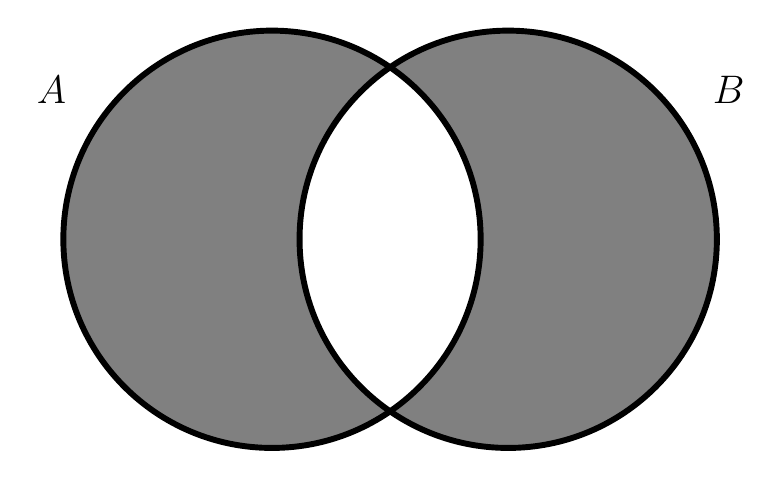
\begin{tikzpicture}
        \def\firstcircle{(-.5,0) circle (2.65cm)}
        \def\secondcircle{(2.5,0) circle (2.65cm)}
        
        % Fill the symmetric difference
        \fill[even odd rule, gray]\firstcircle \secondcircle;
        
        % Draw the circle outlines and add labels
        \draw[draw=black,line width=.75mm] \firstcircle;
        \draw[draw = black, line width=.75mm] \secondcircle;
        \node at (-3.3,1.9) {\Large$A$};
        \node at (5.3,1.9) {\Large$B$};
    \end{tikzpicture}}
    \caption{Set symmetric difference $A\bigtriangleup B$ represented by the gray-shaded region }
    \label{fig:setsim}
\end{figure}
Mathematically, this intuition is described by the notion of continuity
of $J$ in the closed interval $[t, t+1]$ ~(the union of any two balls) and the absolute continuity of $J$ over the interval  $[0,T]$~(the union of all balls in a complete interval) since the notion of these balls is defined dependent on the tasks. We will define measure $\mu$ over the task probability space ~$\mathbb{P}$ and describe an $\varepsilon, \delta$ definition of 
continuity of a function w.r.t this measure defined over the set symmetric difference $\mu(A\bigtriangleup B)$.
\begin{definition} \label{defintersect}
     Let $\overline{\tx} = \bigcup_{t=0}^\infty \tx(t)$ with the power set $\mathcal{P(\overline{\tx})}$ as its topology. Set $\mathcal{B(\overline{\tx})}$ to be the Borel sigma algebra on $\overline{\tx}$ equipped with a probability measure denoted $\mu.$ Then $(\overline{\tx},\mathcal{B}(\overline{\tx}), \mu)$ forms a probability measure space. Let $\hat{f}: \overline{\tx}\rightarrow \mathbb{R}$ be a measurable function, and set $F:\mathcal{B}(\overline{\tx})\rightarrow \mathbb{R}$ to be the function
     \begin{align*}
         F(A) & = \int_{\vx \in A} \fhat(\vx) d\mu,
     \end{align*}
     where $\fhat(\weight(t),\psi(t))( \vx )  = \fhat(\vx)$.
     Then we say that $F$ is \textit{continuous with respect to the measure} if for every $\varepsilon>0$ there exists $\delta >0$ such that $\abs{F(A)-F(B)} < \varepsilon$
     whenever $A,B\in \mathcal{B(\overline{\tx})}$ such that $\mu(A\bigtriangleup B)<\delta.$
 \end{definition}
 
Definition \ref{defintersect} can be deduced from basic measure 
theory results found in \cite{weaver2013measure} implying that 
sets that are similar~(with respect to the probability measure $\mu$) 
result in close values of $F(A)$, integrated over the respective sets. 
In particular, $\mu(A\bigtriangleup B)$ is the Lebesgue measure $\mu$
applied over $A\bigtriangleup B$ representing a set 
symmetric difference, which describes the elements 
two sets do not share~(see Figure  \ref{fig:setsim} 
for an illustration). Therefore, as the intersection space (i.e., $\mu(A\cap B)$) 
shrinks, $\mu(A\bigtriangleup B)$ gets larger, and $\abs{F(A)-F(B)}$ gets larger proportionally, thus providing a measure of continuity 
that is proportional to the number of common elements between the two sets. More common elements imply a smaller value of the measure, and less common elements 
imply a large value of the measure. 
It is straightforward to see that 
$\mu(A\bigtriangleup B)$  is a Radon--Nikodym measure derived from the probability measure $\mu.$



\subsection{Existence}
To begin, we prove that the expected value function, that is, $\int_{\vx\in A}
       \ell(\fhat(\weight,\psi
       )( \vx ) )d\mu$, is continuous with respect to measure $\mu$ when $\mu(A\triangle B)<\delta, \forall A, B \in \overline{\tx}.$ 
\begin{lemma}\label{lem:contMeasure}
    Let $(\overline{\tx},\mathcal{B}(\overline{\tx}), \mu)$ be the measure space as 
    defined in Definition~\ref{defintersect}. 
    Assume that the loss function $\ell$ is continuous 
    and bounded across all tasks, that is, $\forall t \in [0,T].$ 
    Then the expected value function 
    \begin{align}
        E(A) & = \int_{\vx\in A}
       \ell(\fhat(\weight,\psi
       )( \vx ) )d\mu.\\
    \end{align}
    is continuous with respect to measure $\mu$.
\end{lemma}

\begin{proof}
    Suppose that the constant $M_0>0$ is the value that bounds $\ell$ on every task. Let $\varepsilon>0$, and set $\delta = \varepsilon/M_0.$ Further, let $A,B\in \mathcal{B}(\tx)$ such that $\mu(A\triangle B)<\delta.$ By disjoint additivity of $\mu$ and the triangle inequality, we have
    \begin{align*}
        \abs{E(A)-E(B)} & = \vert \int_{\vx\in A}
       \ell(\fhat(\weight,\psi
       )( \vx ) )d\mu - \int_{\vx\in B}
       \ell(\fhat(\weight,\psi
       )( \vx ) )d\mu\vert\\
       & = \vert \int_{\vx\in A\setminus B}
       \ell(\fhat(\weight,\psi
       )( \vx ) )d\mu + \int_{\vx\in A\cap B}
       \ell(\fhat(\weight,\psi
       )( \vx ) )d\mu\\
       & - \int_{\vx\in B\setminus A}
       \ell(\fhat(\weight,\psi
       )( \vx ) )d\mu - \int_{\vx\in A\cap B}
       \ell(\fhat(\weight,\psi
       )( \vx ) )d\mu\vert\\
       & = \vert \int_{\vx\in A\setminus B}
       \ell(\fhat(\weight,\psi
       )( \vx ) )d\mu - \int_{\vx\in B\setminus A}
       \ell(\fhat(\weight,\psi
       )( \vx ) )d\mu\vert\\
       & \leq \int_{\vx\in A\setminus B}
       \abs{\ell(\fhat(\weight,\psi
       )( \vx ) )}d\mu + \int_{\vx \in B\setminus A}
       \abs{\ell(\fhat(\weight,\psi
       )( \vx ) )}d\mu.
    \end{align*}
    Then, by the boundedness of $\ell,$ we have
    \begin{align*}
        \int_{\vx\in A\setminus B}
       \abs{\ell(\fhat(\weight,\psi
       )( \vx ) )}d\mu + \int_{\vx\in B\setminus A}
       \abs{\ell(\fhat(\weight,\psi
       )( \vx ) )}d\mu & \leq M_0\mu(A\setminus B)+M_0\mu(B\setminus A).
    \end{align*}
    Hence,
    \begin{align*}
        M_0\mu(A\setminus B)+M_0\mu(B\setminus A) & = M_0 \mu(A\triangle B)\\
        & <M_0\delta\\
        & = M_0\frac{\varepsilon}{M_0}\\
        & = \varepsilon,
    \end{align*}
    as desired.
\end{proof}
Now we show that two tasks $\tx(t), \tx(t+1)$  when similar~(connected sets) such that $\mu(\tx(t)\bigtriangleup \tx(t+1))<\delta$ imply that $\abs{\clcost-\clcostt}<\varepsilon$ for a small $\varepsilon >0$  with a  $\delta >0.$
We prove this result in the following lemma. 
\begin{lemma}
    Let $(\overline{\tx},\mathcal{B}(\overline{\tx}), \mu)$ be the measure space as 
    defined in Definition~\ref{defintersect}. 
    Assume that the loss function $\ell$ is continuous 
    and bounded across all tasks, that is, $\forall t \in [0,T].$ 
    Define $J$ over a task $\tx(t)$ as
    \begin{align}
        \clcost & =\int_0^t \ea \;  d~\tau  = \int_{\vx\in \bigcup_{\tau=0}^t\tx(\tau)}       \ell(\fhat(\weight(\tau),\psi(\tau))( \vx ) )d\tau . 
    \end{align}
    Let $\varepsilon >0$ and $\delta(\varepsilon)>0$ chosen such that $\ea$ is continuous w.r.t. measure $\mu$.
    Then, if
    $\mu(\bigcup_{\tau = 0}^{t+\Delta t} \tx(\tau)\triangle \bigcup_{\tau = 0}^{t} \tx(\tau))<\delta$ implies 
    $\abs{\clcostt- \clcost} \leq \varepsilon$ with $\Delta t = 1.$
    GAIL - I don't follow the preceding: If XXX less than delta implies YYY -- where is the If... then part?
\end{lemma}

\begin{proof}
    Suppose that the constant $M_0>0$ bounds $\ell$ on every task. 
    Let $\varepsilon>0$, and  set $\delta = \varepsilon/M_0.$  By disjoint additivity of $\mu$ and triangle inequality, we have
    \begin{align*}
       & \left\vert   
       \int_0^{t+\Delta t} \ea d\mu\; d~\tau- 
       \int_0^t \ea d\mu\; d~\tau\right\vert \\
        & = \left\vert \displaystyle\int_{\bigcup_{\tau = 0}^{t+\Delta t} \tx(\tau)} \ell(\hat{f}(\weight,\psi))d\mu- \displaystyle\int_{\bigcup_{\tau = 0}^{t} \tx(\tau)} \ell(\hat{f}(\weight,\psi))d\mu\right\vert \\
        & = \Big\vert \displaystyle\int_{\bigcup_{\tau = 0}^{t+\Delta t} \tx(\tau)\setminus \bigcup_{\tau = 0}^{t} \tx(\tau)} \ell(\hat{f}(\weight,\psi))d\mu+ \displaystyle\int_{\bigcup_{\tau = 0}^{t} \tx(\tau)\cap\bigcup_{\tau = 0}^{t+\Delta t} \tx(\tau)} \ell(\hat{f}(\weight,\psi))d\mu\\
        & -\displaystyle\int_{\bigcup_{\tau = 0}^{t+\Delta t} \tx(\tau)} \ell(\hat{f}(\weight,\psi))d\mu- \displaystyle\int_{\bigcup_{\tau = 0}^{t} \tx(\tau)\cap \bigcup_{\tau = 0}^{t+\Delta t} \tx(\tau)} \ell(\hat{f}(\weight,\psi))d\mu\Big\vert\\
        & = \Big\vert \displaystyle\int_{\bigcup_{\tau = 0}^{t+\Delta t} \tx(\tau)\setminus \bigcup_{\tau = 0}^{t} \tx(\tau)} \ell(\hat{f}(\weight,\psi))d\mu-\displaystyle\int_{\bigcup_{\tau = 0}^{t+\Delta t} \tx(\tau)} \ell(\hat{f}(\weight,\psi))d\mu\Big\vert\\
        & \leq \displaystyle\int_{\bigcup_{\tau = 0}^{t+\Delta t} \tx(\tau)\setminus \bigcup_{\tau = 0}^{t} \tx(\tau)} \abs{\ell(\hat{f}(\weight,\psi))}d\mu-\displaystyle\int_{\bigcup_{\tau = 0}^{t+\Delta t} \tx(\tau)} \abs{\ell(\hat{f}(\weight,\psi))}d\mu \\.
    \end{align*}
    Then, by the boundedness of $\ell,$
    \begin{align*}
        &\displaystyle\int_{\bigcup_{\tau = 0}^{t+\Delta t} \tx(\tau)\setminus \bigcup_{\tau = 0}^{t} \tx(\tau)} \abs{\ell(\hat{f}(\weight,\psi))}d\mu-\displaystyle\int_{\bigcup_{\tau = 0}^{t+\Delta t} \tx(\tau)} \abs{\ell(\hat{f}(\weight,\psi))}d\mu \\
        & \leq M_0 \mu(\bigcup_{\tau = 0}^{t+\Delta t} \tx(\tau)\setminus \bigcup_{\tau = 0}^{t} \tx(\tau)) + M_0\mu(\bigcup_{\tau = 0}^{t} \tx(\tau)\setminus \bigcup_{\tau = 0}^{t+1} \tx(\tau)).
    \end{align*}
    Hence,
    \begin{align*}
        M_0 \mu(\bigcup_{\tau = 0}^{t+\Delta t} \tx(\tau)\setminus \bigcup_{\tau = 0}^{t} \tx(\tau)) + M_0\mu(\bigcup_{\tau = 0}^{t} \tx(\tau)\setminus \bigcup_{\tau = 0}^{t+1} \tx(\tau)) & = M_0\mu(\bigcup_{\tau = 0}^{t+\Delta t} \tx(\tau)\triangle \bigcup_{\tau = 0}^{t} \tx(\tau))\\
        & < M_0\delta\\
        & = M_0 \frac{\varepsilon}{M_0}\\
        & = \varepsilon,
    \end{align*}
    as desired with $\Delta t = 1.$
\end{proof}

%remark justifying loss bounded on all tasks
\begin{remark}\label{boundedremark}
    It is reasonable to assume that there is some constant $M_0<\infty$ for which $M_i\leq M_0$ 
    for all $i\in \mathbb{N}$ because 
    if one did not exist, then the problem would be unsolvable since
    an unbounded loss function would imply that 
    the neural network is not learning anything useful from the data. 
\end{remark}

% remark justifying the union.
\begin{remark}\label{boundedremark}
    The  equality  $\int_0^t \ea \;  d~\tau  = \int_{\vx\in \bigcup_{\tau=0}^t\tx(\tau)}       \ell(\fhat(\weight(\tau),\psi(\tau))( \vx ) )d\tau $ is not always guaranteed because the duplicates among all $\tx(\tau), \forall \tau$  are counted only once. However, we assume that within the construction of $\ell,$ there is an average between all duplications, and only one instance of these duplicates survives. This is reasonable because, in practice, a batch of data is uniformly sampled and averaged over.
\end{remark}

Lemma~\ref{lem:contMeasure} solidifies the notion that similar 
tasks produce similar loss values and that $\clcost$ is continuous with respect 
to the measure $\mu$ for any $ \tx(t), \tx(t+1) \in \mathcal{B}(\overline{\tx}).$  The  lemma provides the conditions for when a solution between two consecutive tasks  exists. If  Lemma~\ref{lem:contMeasure} is upheld for every $t \in [0,T],$, then the CL problem will have a solution for the whole interval $[0,T].$ To provide a rigorous notion of this, we have the following definition.
\begin{definition}
    \label{defabsolutely_continuous}
     Consider the interval $[0,T]$ and  $\overline{\tx} = \bigcup_{t=0}^T \tx(t)$ with the power set $\mathcal{P(\overline{\tx})}$ as its topology. Set $\mathcal{B(\overline{\tx})}$ to be the Borel sigma algebra on $\overline{\tx}$ equipped with a probability measure  $\mu.$ Then, $(\overline{\tx},\mathcal{B}(\overline{\tx}), \mu)$ forms a probability measure space. Define the set $[0,T] = [0,1] \cup  (1, 2], \cdots (t, t+1], \cdots, \cup, \cdots, \cup, (T-1, T].$  Let $\hat{f}: \overline{\tx}\rightarrow \mathbb{R}$ be a measurable function. For any 
     $t \in [0,T],$ define $F(t):\mathcal{B}(\overline{\tx}) \rightarrow \mathbb{R}$ such that  $F(t) = \int_0^t \ea \;  d~\tau$. If  $\sum_{t}^{T} \mu((\tx(\tau+1)\cup \tx(\tau)) \bigtriangleup \tx(\tau+1))<\delta$ implies $\sum_{t}^{T} \left\vert F(t)-F(t+1) \right\vert \leq \varepsilon,$ then $F$ is absolutely continuous over the interval $[t,T].$
 \end{definition}
With this definition and the notation that $E(\tx(\tau)) = \ea$ we have the following theorem.
\begin{theorem}\label{thm:contMeasure}
    Let $(\overline{\tx},\mathcal{B}(\overline{\tx}), \mu)$ be the measure space as 
    defined  in Definition~\ref{defintersect} and requirements for absolute continuity defined as in Definition~\ref{defabsolutely_continuous}. Assume that the loss function $\ell$ is continuous 
    and bounded for all tasks, that is, $\forall t \in [0,T].$ 
    Define $J$ over a task $\tx(\tau)$ as
    \begin{align}
   \clcost & = \int_0^t  E(\tx(\tau)) \;  d~\tau .
    \end{align}
    Then $ \clcost$ is absolutely continuous with respect to the measure for all $\{ \tx(\tau) \in \mathcal{B}(\overline{\tx}), \tau =0,1, \cdots, t \}.$
\end{theorem}
\begin{proof}
    Suppose that the constant $M_0>0$ bounds $\ell$ on every task. 
    Let $\varepsilon>0$, and  set $\delta = \varepsilon/TM_0.$ 
    Furthermore, let $\tx(t+1),\tx(t) \in \mathcal{\mathcal{B}}(\overline{\tx})$ 
    such that $\mu(\bigcup_{\tau = 0}^{t+\Delta t} \tx(\tau)\triangle \bigcup_{\tau = 0}^{t} \tx(\tau))< \delta.$  Then, by the boundedness of $\ell$ and from Lemma~\ref{lem:contMeasure} and Theorem~\ref{thm:contMeasure} with the choice of $\delta = \frac{\varepsilon}{2(T-t) M_0},$ we have
    \begin{align*}
        & \sum_{t}^T \left[ \left\vert J(\weight(\tau+\Delta \tau),\psi(\tau+\Delta \tau),\tx(\tau+\Delta \tau)) - \clcost \right\vert \right] \\ 
        & \leq \sum_{t}^T \left\vert M_0 \mu(\bigcup_{\tau = 0}^{t+\Delta t} \tx(\tau)\triangle \bigcup_{\tau = 0}^{t} \tx(\tau)) \right\vert 
        + \left\vert M_0  \mu\left(\bigcup_{\tau = 0}^{t+\Delta t} \tx(\tau)\triangle \bigcup_{\tau = 0}^{t} \tx(\tau)) \right) \right\vert \\
        & \leq \sum_{t}^T M_0( \frac{\varepsilon}{ (T-t) 2M_0} + \frac{\varepsilon}{2(T-t) M_0} ),
    \end{align*}
    which gives the result according to Definition~\ref{defabsolutely_continuous}.
\end{proof}
Therefore, the existence of a solution to \eqref{eq:clcum} depends on whether we can ensure absolute continuity of $\int_0^t \ea \;  d~\tau$ or not. 

\subsection{Reachability to a Solution in the Presence of Dissimilar Tasks}
Theorem~\ref{thm:contMeasure} shows the condition of existence of the CL solution for \eqref{eq:clcum}. 
The contrapositive reveals that dissimilar loss values imply dissimilar tasks.  For an arbitrary CL problem, however,
dissimilar tasks may or may not result in dissimilar loss values. 
That is, if we have two tasks $\tx(t)$ and $\tx(t+\Delta t)$ 
such that $\mu \left( \tx(t)\bigtriangleup \tx(t+\Delta t) \right) \geq \delta$, 
 we do not know whether $\abs{\clcost-\clcostt} \leq \varepsilon$ 
(i.e., similar loss values) or $\abs{\clcost-\clcostt} \geq \varepsilon$ 
(i.e., dissimilar loss values).
Nonetheless, if dissimilar tasks do produce dissimilar loss values and the number of tasks increases, the value of $\abs{\clcost-\clcostt}$ will tend to increase  and eventually exceed $\varepsilon.$
Therefore, the model will gradually forget prior tasks, and eventually CL will fail, thus violating Theorem~\ref{thm:contMeasure}. 

In order to counteract this situation, the key condition for absolute continuity must be upheld; that is, for a series of tasks, the upper bound on 
$ \sum_{t}^T \left[ \left\vert J(\weight(\tau+\Delta \tau),\psi(\tau+\Delta \tau),\tx(\tau+\Delta \tau)) - \clcost \right\vert \right]$ must be guaranteed to be less than or equal to $\varepsilon$. The key here is to identify the knobs in the model that can be tuned to ensure that $\varepsilon$ is small even in the presence of dissimilar tasks. In the typical neural network learning problem, the two knobs that can be tuned are the weights and architecture of the network. We will cement these ideas in the following and begin by elucidating the dependency of $\ea$ on the weights and the architecture.

% \Ally{I don't know that we can find a lower bound which we can guarantee is nonnegative. This is because we can't estimate inside the bigger absolute values introduced by the reverse triangle inequality. Yes, we can remove the outer set of absolute values, but this is where we gain the issue having a negative lowerbound. Beyond the concern of the lower bound not being negative, I don't think we will be able to show the lower bound pushes up (goes to infinity) because $\mu(\tx(t)\triangle \tx(t+1))\geq \delta$ does not guarantee that we don't have similar loss values (as you note in the paragraph above). I believe this is why I can't get this to work. Below is the lower bound I can get, but cannot guarantee nonnegative. \newline However, I don't know that an upperbound doesn't make equal amount of sense. We find an upperbound $C$ on $|J-J|$ when we change only the weights.  We can then find a smaller upper bound $C'$ on $|J-J|$ when we change architecture and weights. Thus, if $|J-J|\geq \varepsilon$ (i.e. dissimilar loss value), then, we know $C\geq |J-J|\geq \varepsilon,$ but by also changing the architecture we have $C\geq C'\geq |J-J|.$ This can result in $|J-J|< \varepsilon$ (i.e. similar loss value) since we can have $|J-J|\leq C'<\varepsilon<C.$\newline I am hesitant to frame this section through the lens of "absolutely continuous" or "not absolutely continuous" because $\mu(\tx(t)\triangle \tx(t+1))\geq \delta.$ We can't shrink $\mu(\tx(t)\triangle \tx(t+1))$ because the data is fixed. So, we can't say by changing the architecture and the weights that it is now "absolutely continuous." Yes, perhaps "shrinking" $\varepsilon$ could lead to a new (bigger) $\delta$ choice, but we don't know that. We only have that for every epsilon there is a delta.}

%=============Taylor Theorem weights and arch=========%
\begin{lemma}\label{lem:taylor}
    Suppose $\tx(t)$ and $\tx(t+\Delta T)$ are two consecutive tasks in the measure space $(\overline{\tx}, \mathcal{B}(\overline{\tx}),\mu).$  Set $M_0$ to be the upper bound on the loss function $\ell$ across all tasks. Then for $\mu(\tx(t)\bigtriangleup \tx(t+\Delta t))\geq \delta,$ the following holds:
    \begin{align}
        E\left(\bigcup_{\tau = 0}^{t+1}\tx(\tau)\right) & = E\left(\bigcup_{\tau = 0}^{t}\tx(\tau)\right) + \Delta t\Big[\mu\left( \bigcup_{\tau = 0}^{t}\tx(\tau)\Delta \bigcup_{\tau = 0}^{t+1}\tx(\tau)\right)\cdot \displaystyle\int_{\bigcup_{\tau = 0}^{t}\tx(\tau)\Delta \bigcup_{\tau = 0}^{t+1}\tx(\tau)} \ell(\hat{f}(\weight,\psi))d\mu \nonumber \\
        & + \displaystyle\int_{\bigcup_{\tau = 0}^{t}\tx(\tau)} \ell'(\hat{f}(\weight,\psi))\cdot \partial_{\weight}^1 \hat{f}(\weight,\psi)\cdot \Delta w \hspace{1mm} d\mu \nonumber \\
        & +\displaystyle\int_{\bigcup_{\tau = 0}^{t}\tx(\tau)} \ell'(\hat{f}(\weight,\psi))\cdot \partial_\psi^1 \hat{f}(\weight,\psi)\cdot \Delta \psi \hspace{1mm}  d\mu\Big]+ o(\Delta t).\label{archfinaltaylor}
    \end{align}
\end{lemma}
\begin{proof}
    Note that the first-order Taylor series expansion of $E(\tx(t+\Delta t))$ about  $t$ is given by
    \begin{align}
        E\left(\bigcup_{\tau = 0}^{t+1}\tx(\tau)\right) & = E\left(\bigcup_{\tau = 0}^{t}\tx(\tau)\right) + \Delta t\Big[ E_{\tx} \left(\bigcup_{\tau = 0}^{t+1}\tx(\tau)\Delta \bigcup_{\tau = 0}^{t}\tx(\tau)\right) \nonumber \\
        & + E_{\weight}\left(\bigcup_{\tau = 0}^{t}\tx(\tau)\right) + E_\psi\left(\bigcup_{\tau = 0}^{t+1}\tx(\tau)\right)\Big] + o(\Delta t),\label{taylorexparch}
    \end{align}
    where $E_{\tx} , E_{\weight},$ and $E_\psi$ are the partial derivatives of the expected value function for the data, weights, and architecture, respectively. Now, we work on acquiring each partial derivative. Toward that end, 
    \begin{align}
        E_{\tx} \left(\bigcup_{\tau = 0}^{t+1}\tx(\tau)\Delta \bigcup_{\tau = 0}^{t}\tx(\tau)\right) & =\mu\left( \left(\bigcup_{\tau = 0}^{t+1}\tx(\tau)\Delta \bigcup_{\tau = 0}^{t}\tx(\tau)\right)\right)\cdot \displaystyle\int_{\left(\bigcup_{\tau = 0}^{t+1}\tx(\tau)\Delta \bigcup_{\tau = 0}^{t}\tx(\tau)\right)} \ell(\hat{f}(\weight,\psi))d\mu.\label{E_X1}
    \end{align}
    To determine the remaining two derivatives, we use the Sobolev function chain rule found in \cite{evans2022partial}. We can do so because $\ell$ is real-valued and bounded and $\ell'$ is continuously differentiable. Then,
    \begin{align}
        E_{\weight}\left(\bigcup_{\tau = 0}^{t}\tx(\tau)\right) & = \displaystyle\int_{\bigcup_{\tau = 0}^{t}\tx(\tau)} \ell'(\hat{f}(\weight,\psi))\cdot \partial_{\weight}^1 \hat{f}(\weight,\psi)\cdot \Delta w \hspace{1mm}  d\mu.\label{E_w},\\
        E_{\psi}\left(\bigcup_{\tau = 0}^{t}\tx(\tau)\right) & = \displaystyle\int_{\bigcup_{\tau = 0}^{t}\tx(\tau)} \ell'(\hat{f}(\weight,\psi))\cdot \partial_\psi^1 \hat{f}(\weight,\psi)\cdot \Delta \psi \hspace{1mm}  d\mu.\label{E_psi}
    \end{align}
    Substituting (\ref{E_X1}), (\ref{E_w}), and (\ref{E_psi}) into the Taylor series expansion (\ref{taylorexparch}), we have
    \begin{align*}
        E\left(\bigcup_{\tau = 0}^{t+1}\tx(\tau)\right) & = E\left(\bigcup_{\tau = 0}^{t}\tx(\tau)\right) + \Delta t\Big[\mu\left( \bigcup_{\tau = 0}^{t}\tx(\tau)\Delta \bigcup_{\tau = 0}^{t+1}\tx(\tau)\right)\cdot \displaystyle\int_{\bigcup_{\tau = 0}^{t}\tx(\tau)\Delta \bigcup_{\tau = 0}^{t+1}\tx(\tau)} \ell(\hat{f}(\weight,\psi))d\mu\\
        & + \displaystyle\int_{\bigcup_{\tau = 0}^{t}\tx(\tau)} \ell'(\hat{f}(\weight,\psi))\cdot \partial_{\weight}^1 \hat{f}(\weight,\psi)\cdot \Delta w \hspace{1mm} d\mu \\ &+\displaystyle\int_{\bigcup_{\tau = 0}^{t}\tx(\tau)} \ell'(\hat{f}(\weight,\psi))\cdot \partial_\psi^1 \hat{f}(\weight,\psi)\cdot \Delta \psi \hspace{1mm}  d\mu\Big] \\ &+ o(\Delta t).
    \end{align*}
\end{proof}

Colloquially, in the CL problem only the weights are updated, but in this paper we argue that this is not enough. We show that  with just the weights being updated, the $\clcost$ eventually violates Theorem~\ref{thm:contMeasure}. To prove this, we first derive a lower bound on $\ea.$ For the remaining analysis, we will set  $ \Delta t = 1.$

%--------------New upperbound weights -------------------%
\begin{lemma}\label{lem:upper_weight}
    Suppose $\tx(t)$ and $\tx(t+\Delta t)$ are two consecutive tasks in the measure space $(\overline{\tx}, \mathcal{B}(\overline{\tx}),\mu).$ Let $L_1>0$ and $0\leq \delta\leq 1$  be constants. Set $M_0$ to be the upper bound on the loss function $\ell$ across all tasks, and assume $\mu\left( \bigcup_{\tau = 0}^{t}\tx(\tau)\Delta \bigcup_{\tau = 0}^{t+\Delta t}\tx(\tau)\right)\geq \delta$ for all $t\in [0,T].$ Then for $\Delta t = 1$ the following holds:
    \begin{align*}
        \sum_{\tau = t}^{T} \left(J(\tx(\tau))-J(\tx(\tau+1)\right)
        & \leq \sum_{\tau =t}^{T} \Big( M_0\cdot \delta - \displaystyle\int_{\bigcup_{\nu = 0}^\tau\tx(\nu)} \left(\ell'(\hat{f}(\weight,\psi))\cdot \partial_{\weight}^1 \hat{f}(\weight,\psi)\right)^2 \hspace{1mm}  d\mu \Big)
    \end{align*}
    for $\displaystyle\int_{\tx(t)} \ell'(\hat{f}(\weight,\psi))\cdot \partial_\psi^1 \hat{f}(\weight,\psi)\cdot \Delta \psi \; \;  d\mu+ o(\Delta t) = 0$ as $\psi(t) = \psi, \forall t.$
\end{lemma}
\begin{proof}
    The proof is in Section~\ref{sec:upper_weight}.
\end{proof}
A bound similar to the one in Lemma~\ref{lem:upper_weight} can be attained for the architecture terms as well. 
%--------------New upperbound weights and arch -------------------%
\begin{lemma}\label{lem:upper_arch}
    Suppose $\tx(t)$ and $\tx(t+\Delta t)$ are two consecutive tasks in the measure space $(\overline{\tx}, \mathcal{B}(\overline{\tx}),\mu).$ Let $L_1>0$ and $0\leq \delta\leq 1$  be constants. Set $M_0$ to be the upper bound on the loss function $\ell$ across all tasks, and assume $\mu\left( \bigcup_{\tau = 0}^{t}\tx(\tau)\Delta \bigcup_{\tau = 0}^{t+\Delta t}\tx(\tau)\right)\geq \delta$ for all $t\in [0,T].$ Then for $\Delta t = 1$ the following holds:
    \begin{align*}
        \sum_{\tau = t}^{T} \left(J(\tx(\tau))-J(\tx(\tau+1)\right)
        & \leq \sum_{\tau =t}^{T} \Big( M_0\cdot \delta - \displaystyle\int_{\bigcup_{\nu = 0}^\tau\tx(\nu)} \left(\ell'(\hat{f}(\weight,\psi))\cdot \partial_{\weight}^1 \hat{f}(\weight,\psi)\right)^2 \hspace{1mm}  d\mu\\
        & -\displaystyle\int_{\bigcup_{\nu = 0}^\tau\tx(\nu)} \left(\ell'(\hat{f}(\weight,\psi))\cdot \partial_\psi^1 \hat{f}(\weight,\psi)\right)^2\hspace{1mm}  d\mu\Big).
    \end{align*}
\end{lemma}
\begin{proof}
    The proof is  in Section~\ref{sec:upper_arch}.
\end{proof}

The following result tells us that in the case of dissimilar tasks and with dissimilar loss values ($\sum_{\tau = t}^{T} \left(J(\tx(\tau)) - J(\tx(\tau+1))\right)\geq \varepsilon)$ for a fixed architecture across tasks, we can learn the architecture at each task such that we can acquire similar loss values tasks ($\sum_{\tau = t}^{T} \left(J(\tx(\tau)) - J(\tx(\tau+1))\right) < \varepsilon).$ 
\begin{theorem}\label{thm:intersection}
    Let $\varepsilon >0$, and choose $\delta$ $J$ to be absolutely continuous.
    Suppose $\tx(t)$ and $\tx(t+\Delta t)$ are two consecutive tasks in the measure space $(\overline{\tx}, \mathcal{B}(\overline{\tx}),\mu).$ Set $M_0$ to be the upper bound on the loss function $\ell$ across all tasks, and assume $\mu\left( \bigcup_{\tau = 0}^{t}\tx(\tau)\Delta \bigcup_{\tau = 0}^{t+1}\tx(\tau)\right)\geq \delta$ for all $t\in [0,T].$ If for a fixed architecture $\psi^*$ for all $t\in [0,T]$
    \begin{align*}
        \sum_{\tau = t}^{T} \left(J(\weight(\tau), \psi^*, \tx(\tau)) - J(\weight(\tau+1), \psi^*, \tx(\tau+1))\right) & \geq \varepsilon,
    \end{align*}
    then we can choose a new architecture $\psi(t)$ for $[0,T]$ such that we can have
    \begin{align*}
        \sum_{\tau = t}^{T} \left(J(\weight(\tau), \psi^*, \tx(\tau)) - J(\weight(\tau+1), \psi(\tau), \tx(\tau+1))\right) & < \varepsilon.
    \end{align*}
\end{theorem}

\begin{proof}
    Let $\varepsilon >0$, and choose $\delta$ $J$ to be absolutely continuous. As
    \begin{align*}
        \displaystyle\int_{\bigcup_{\nu = 0}^\tau\tx(\nu)} \left(\ell'(\hat{f}(\weight,\psi))\cdot \partial_{\psi}^1 \hat{f}(\weight,\psi)\right)^2 & >0,
    \end{align*}
    notice that
    \begin{align*}
         \sum_{\tau = t}^{T} \left(J(\tx(\tau)) - J(\tx(\tau+1))\right)
        & \leq \sum_{\tau =t}^{T} \Big( M_0\cdot \delta - \displaystyle\int_{\bigcup_{\nu = 0}^\tau\tx(\nu)} \left(\ell'(\hat{f}(\weight,\psi))\cdot \partial_{\weight}^1 \hat{f}(\weight,\psi)\right)^2 \hspace{1mm}  d\mu\\
        & -\displaystyle\int_{\bigcup_{\nu = 0}^\tau\tx(\nu)} \left(\ell'(\hat{f}(\weight,\psi))\cdot \partial_{\psi}^1 \hat{f}(\weight,\psi)\right)^2 \hspace{1mm}  d\mu \Big)\\
        & \leq \sum_{\tau =t}^{T} \Big( M_0\cdot \delta - \displaystyle\int_{\bigcup_{\nu = 0}^\tau\tx(\nu)} \left(\ell'(\hat{f}(\weight,\psi))\cdot \partial_{\weight}^1 \hat{f}(\weight,\psi)\right)^2 \hspace{1mm}  d\mu \Big).
    \end{align*}
    Thus, by changing the architecture we may be able to achieve
    \begin{align*}
         \sum_{\tau = t}^{T} \left(J(\tx(\tau)) - J(\tx(\tau+1))\right)
        & \leq \sum_{\tau =t}^{T} \Big( M_0\cdot \delta - \displaystyle\int_{\bigcup_{\nu = 0}^\tau\tx(\nu)} \left(\ell'(\hat{f}(\weight,\psi))\cdot \partial_{\weight}^1 \hat{f}(\weight,\psi)\right)^2 \hspace{1mm}  d\mu\\
        & -\displaystyle\int_{\bigcup_{\nu = 0}^\tau\tx(\nu)} \left(\ell'(\hat{f}(\weight,\psi))\cdot \partial_{\psi}^1 \hat{f}(\weight,\psi)\right)^2 \hspace{1mm}  d\mu \Big)\\
        & <\varepsilon\\
        & \leq \sum_{\tau =t}^{T} \Big( M_0\cdot \delta - \displaystyle\int_{\bigcup_{\nu = 0}^\tau\tx(\nu)} \left(\ell'(\hat{f}(\weight,\psi))\cdot \partial_{\weight}^1 \hat{f}(\weight,\psi)\right)^2 \hspace{1mm}  d\mu \Big).
        \end{align*}
    Thus, we have reduced the difference in loss values below the $\varepsilon$ threshold to gain similar loss values when we began with dissimilar tasks.
\end{proof}
The implications of Theorem~\ref{thm:intersection} indicate that it is possible to shrink the effect of the new task on the forgetting cost $J$ by changing the architecture of the network by pushing $\varepsilon$ closer to zero. The closer $\varepsilon$ is to zero, the more the cardinality of the intersection space and the more the task sets are connected. Therefore, upholding the absolute continuity of $J$ is feasible. 

It is now of interest to identify how to change the architecture and efficiently learn over a series of tasks. In particular, we must examine to what extent we can control the effect of architecture change on the CL problem. 


\begin{figure}
    \centering
    \includegraphics[width=\linewidth]{paperFigures/intersect22.png}
    \caption{CL solution, where we change the size of the intersection space by introducing more capacity, through choosing novel hyperparameters}
    \label{fig:solution}
\end{figure}
\section{CL Solution}
To understand how to change the architecture of the model and learn over a series of tasks within the CL paradigm, we consider Figure~\ref{fig:solution}. We begin at task $t = 1$ and determine an optimal weight denoted $w^*(1) = w^\infty(1).$ This gives us a neural network solution in $\mathcal{F}_1.$ Then, as the next task is observed, we perform a derivative-free hyperparameter search, in particular, the directional direct search method~\cite{larson2019derivative}, to obtain a new architecture. The solution to this search is denoted $\psi^\infty(2)$ as in  Figure ~\ref{fig:solution}. Notably,  a new quandary arises since the new architecture introduces a parameter space that may have a different size from the one used for the previous task. Unfortunately, it is not feasible to trivially transfer information from the previous architecture to the new one. The common and state-of-the-art solution to this problem is to initialize the parameters in the new architecture from random and retrain on all available tasks, which is resource heavy as well as impractical. Instead, we develop a low-rank transfer algorithm that seeks to transfer information between the previous architecture to the new architecture in an efficient way. Mathematically, our goal is to solve the following bi-level problem:
\begin{align}\label{eq:bilevel} \tag{bi-level}
     V^*(t,\weight(t))  = \min_{\weight \in \mathcal{W}(\psi^*(t))} V(t,\weight(t)),\quad \text{ where}\; \;  \psi^*(t)  = \mathrm{arg}\min_{\psi\in \Psi} J(\weight(t),\psi,\tx(t)).
\end{align}
Noting that the weight search space at each $t$ is a function of the optimal architecture, we change the weights from $t\rightarrow t+\Delta~t$ as 
\begin{align}
    \weight(t+\Delta~t) = \mathrm{A}^*(t) \weight(t) \mathrm{B}(t)^{*T},
\end{align}
where $\mathrm{A}$ and $\mathrm{B}$ are matrices that enable the transfer of information between two different parameter spaces and where $\mathrm{A}^*, \mathrm{B}^*$ are the optimal values such that loss of information is minimal. This change in the weight space for each new task introduces dynamics into the continual learning problem defined by $V^*.$ The following result therefore provides the total variation~(the dynamics) in $V^*$ as a function of tasks.
\begin{proposition}\label{HJB}
    The total variation in $V^*(t)$ at any given task $t$ is given by
    \begin{align}\label{eq:HJB}
        -\partials_t V^*(t)& = \min_{\weight \in \mathcal{W}(\psi^*(t))} J(\weight(t),\psi^*(t),\tx(t)) + \partials_{\tx}d_{t} \tx+ \partials_{\weight} V^*(t) \left[\mathrm{A}^*(t)\weight(t)( \mathrm{B}^*(t))^T + u(t)\right],
    \end{align}
    where $\mathrm{A}^*(t),B^*(t)$ are optimal $\mathrm{A}(t)$ and $\mathrm{B}(t)$ for task $t$ and where $u(t)$ represents the updates made to the each weights matrix of the new dimensions. 
\end{proposition}
\begin{proof}
    The proof is in Section~\ref{sec:HJB}.
\end{proof}

Observe that \eqref{eq:HJB} is missing the term $\frac{\partials V^*}{\partials \psi}\frac{\partials \psi}{\partials t}.$ This omission is intentional because the exact effects of architecture cannot be measured through derivatives in this partial differential equation (PDE). Instead, in this PDE the effect is absorbed through the change in tensors $\mathrm{A}(t)$ and $\mathrm{B}(t)$.
Because of this absorption we can now define a lower bound on $\partials_{t} V^*(t).$ This lower bound, which is essentially a lower bound on the variation, is equivalent to the lower bound on $\varepsilon$ in Theorem~\ref{thm:intersection} with the distinction that the lower bound is derived on $V^*$ instead of just the forgetting cost $J.$ The idea covers the effects of the dynamic program. We derive this bound below.

\begin{theorem}\label{thm:lower_HJB}
Given proposition~\ref{HJB}, assume there exists a stochastic-gradient-based optimization procedure,  and choose $ u(t) =- \sum^{I} \alpha(i) \mathrm{g}^{(i)},$ where $I$ is the number of updates and $\alpha(i)$ is some learning rate. Choose $\alpha(i)$ such that $\norm{\mathrm{g}_{\mathrm{MIN} }}  \norm{\sum^{I} \alpha(i) } \rightarrow 0$ as $I \rightarrow \infty$ and $\min_{\weight \in \mathcal{W}(\psi^*(t))} J(\weight(t),\psi^*(t),\tx(t)) \leq \varepsilon.$ Then, as long as the architecture is chosen such that $   \sing \delta = \left[ \singmin \norm{\mathrm{g}_{\mathrm{MIN} }}  \norm{\sum^{I} \alpha(i) } - \singw \norm{\mathrm{A}^*(t)\weight(t)( \mathrm{B}^*(t))^T} \right],$  the total variance in $V^*$ is bounded by $\varepsilon.$ 
\end{theorem}
\begin{proof}
    The proof is in Section~\ref{sec:lower_HJB}.
\end{proof}
Therefore, even when $\alpha(i)$ is chosen such that $\norm{\mathrm{g}_{\mathrm{MIN} }}  \norm{\sum^{I} \alpha(i) } $ as $I \rightarrow \infty,$ $\sing \delta$ can be countered by 
$\singw \norm{\mathrm{A}^*(t)\weight(t)( \mathrm{B}^*(t))^T}$, and this bound is tunable because of the change in the architecture. Therefore, as long as $\singw \norm{\mathrm{A}^*(t)\weight(t)( \mathrm{B}^*(t))^T} = \sing \delta$, the total variance is bounded for all $t$. With the presence of bounded variance across all $t$, the sum of these variances is bounded. Therefore, it is clear that the $V^*$ is absolutely continuous as long as $\varepsilon$ is small for all $\delta >0.$
\begin{remark}
    Theorem~\ref{thm:lower_HJB} is crucial because it shows that, in the presence of a perfect stochastic gradient algorithm, the change in the tasks can be countered by the choice of the architecture. By choosing a new architecture and introducing the $A$ and $B$ matrices such that within the CL problem the effect of varying data distribution can be mitigated,  the CL problem can be acceptably solved.
\end{remark}


Given this guarantee, the rest of this section is dedicated to constructing an algorithm such that the condition to ensure this bounded variance is satisfied. In summary~(refer to Figure~\ref{fig:method}), for every new task, we utilize an off-the-shelf algorithm to search for a new optimal architecture. Once a new architecture is found,  we complete a low-rank transfer from the previous task's optimal weights to the new task parameter space. Then, using an off-the-shelf continual learning algorithm, we train the new architecture for the new task while balancing memory on all the prior tasks.  In the process of low-rank transfer, we guarantee transfer of learning by requiring that the $\partials_{t} \leq \eta$, allowing for the intersection of the neural network search spaces between subsequent tasks to increase. Thus, our algorithm comprises three components: step 1 --  architecture search, step 2 --  low-rank transfer, and step 3 --  continual learning. While step 3 is directly adapted from \cite{chakraborty2025understanding, raghavan2021formalizing}, steps 1 and 2 are novel contributions for this work.
\begin{figure}
    \centering
    \includegraphics[width=1.1\linewidth]{paperFigures/method.png}
    \caption{How we do this?}
    \label{fig:method}
\end{figure}


\subsection{\underline{Step 1:}  Architecture Search}\label{archsearch}

Although there are numerous architecture search methods that we could employ, we chose a derivative-free approach that completes a local search using finite difference approximations. This choice was made to mimic the weak derivatives available to us from viewing neural networks as functions of Sobolev spaces. As will become evident in Section \ref{HJB}, a notion of the change in the architecture is needed in order to model the dynamics and solve the lower optimization. We call the search method used a neighborhood directional direct-search (NDDS). The standard directional direct-search method is described in the survey in  \cite{larson2019derivative}. 


The intuition behind NDDS is that we check ``neighboring" architectures and compare the current architecture with the expected value of the neural network when it trains on the neighboring architecture. If the neighboring architecture has a smaller expected value,
then we ``move" in that direction by selecting it as the new architecture. We then check the ``neighbors" of this new architecture. Since the architecture is a discrete variable, this search method provides a notion of a ``gradient." 

With this intuition, we now describe NDDS in depth. As we discuss this method, consult Algorithm \ref{DDSalg}. For task $t\in \tT,$ we set $\tx = \mathcal{Y}$ to be our training data and $J(\weight(t),\psi(t), \mathcal{Y})$ the expected value function. We set $x_s = \psi(t)$, and let $D_s$ be a finite set of directions. Further, we choose a ``step size" $\alpha_s\in \mathbb{N}.$ Now we generate the ``neighboring" points for $x_s$ via $D_s$ and $\alpha_s.$ We call these points \textit{poll points} and define them as follows:
\begin{align*}
    Poll Points = \{x_s + \alpha_s d_i:d_i\in D_s\}.
\end{align*}
Using a randomly selected subset of our data, denoted $\mathcal{Y}_s,$ we determine and compare the expected value of the neural network with randomly initialized weights according to each poll point architecture. If one of these poll points results in a smaller expected value than $x_s,$ we set $x_s$ equal to the poll point. We then repeat this process starting with this new architecture. This search terminates when the expected value is beneath a previously chosen threshold or after five times of repeating. In practice, we chose the threshold to be a percentage lower than the expected value produced by the original architecture.
% \KR{Allyson, wasnt there a nice diagram you had to illustrate this?}

Let us walk through an example. Suppose we would like to learn the optimal number of neurons per layer in our hidden layers for training a feedforward neural network (FNN) on a dataset. Because of the data, suppose the input layer is fixed at $784$ neurons and the output layer is fixed at $10$ neurons per layer. Let us fix the number of hidden layers at $2$ beginning with $50$ neurons in each hidden layer. We set $\mathcal{Y}_s$  to be a randomly chosen appropriately sized subset of task $t$ data and previous task data. Our direction set is $D_s = D = \{[0,0,10,0],[0,10,0,0]\}$ and will be the same for every $s.$ We start our search by setting the step size $\alpha_s = 10.$ For the first round, we have $x_s = [784,50,50,10],$ so our poll points are $[784,60,50,10],[784,50,60,10],$ and $[784,60,60,10].$ We then train an FNN of each size on the dataset $Y_s$ and determine the corresponding expected values. If the expected value of the FNN $[784,60,50,10]$ is smaller than that of the FNN $[784,50,50,10],$ for example, then $x_s = [784,60,50,10].$ We would then continue this process until the expected value of our network was less than our set threshold or we exhausted our neighborhood search. 


% \begin{algorithm}\label{DDSalg}
% \caption{Neighborhood Direct-Directional Search (NDDS)}
% Choose architecture initial point $x_s,$ and step size $\alpha_0\in \mathbb{N}$\\
% Set step parameters
% $\mathrm{threshold}\in \mathbb{R}$\\
% j = 0\\
%  loss $\gets \texttt{training\_loop}(x_s,Y_s)$\\
%  \While{$\mathrm{loss}>\mathrm{threshold}$ or $j<5$}
%     {pollPoints = $\{x_s+\alpha_sd_i:d_i\in D_s\}$\\
%         \For{ $\mathrm{poll\, in\, pollPoints}$}{
%         loss_s $\gets$ \texttt{training\_loop} $(\mathrm{poll},\mathcal{Y}_s)$\\
%       \eIf{$\mathrm{loss}\leq \mathrm{loss}_s$}{
%        $x_{s} = x_s$\;
%        }{
%        $x_{s} = \mathrm{poll}$\;
%        $\mathrm{loss} = \mathrm{loss}_s$\\
%       }
      
%       } $j= j+1;$ }
% \end{algorithm}

\begin{algorithm}[t]
\caption{Neighborhood Directional Direct Search (NDDS)} \label{DDSalg}
\textbf{GAIL - Please decide here and throughout whether you are talking about a neighborhood direct-directional search, a direct-directional neighborhood search, or neighborhood directional direct search}
\KwIn{Initial architecture $x_s$, step size $\alpha_0 \in \mathbb{N}$}
\KwIn{Threshold parameter $\mathrm{threshold} \in \mathbb{R}$}
\KwOut{Updated architecture $x_s$}

$j \gets 0$\;
$\mathrm{loss} \gets \texttt{training\_loop}(x_s, \mathcal{Y}_s)$\;
\While{$\mathrm{loss} > \mathrm{threshold}$ \textbf{or} $j < 5$}{
    $\mathrm{pollPoints} \gets \{x_s + \alpha_s d_i : d_i \in D_s\}$\;
    \ForEach{$\mathrm{poll} \in \mathrm{pollPoints}$}{
        $\mathrm{loss}_s \gets \texttt{training\_loop}(\mathrm{poll}, \mathcal{Y}_s)$\;
        \eIf{$\mathrm{loss} \leq \mathrm{loss}_s$}{
            $x_s \gets x_s$\;
        }{
            $x_s \gets \mathrm{poll}$\;
            $\mathrm{loss} \gets \mathrm{loss}_s$\;
        }
    }
    $j \gets j + 1$\;
}
\end{algorithm}



\subsection{\underline{Step 2:}  Low-Rank Transfer}\label{LRTsec}

Now that the optimal architecture (i.e., number of neurons per layer) has been determined for the current task, it is immediately obvious that  the size of the weights tensor will not match with the new architecture. Thus, we seek a method to determine a weights tensor corresponding to the new optimal architecture that retains previously learned information and transfers it. We propose a method we call low-rank transfer. 

Before we dive into the steps of this method, let us set some assumptions and notation. Recall that the only component of the architecture we seek to learn is the number of neurons per layer in our neural network. Thus, we assume our network has $d$ layers, and we fix all other architecture parameters except for the number of neurons in our hidden layers. From  Definition \ref{defn:NN},  $\psi_i(t)$  provides the dimensions for the corresponding weights matrix in each layer of our network.

In order of appearance, we assign the values of $\psi(t)$ to the values $r_i,s_i$ for each $i$ such that $1\leq i\leq d.$ If $\psi^*(t)$ represents the optimal architecture returned from the NDDS completed for task $t,$ then similarly we can assign the values of the dimensions of the weights matrices of each layer of $\psi_i^*(t)$ to be $a_i,b_i$ for $1\leq i\leq d.$ Our goal is to utilize the original weights matrices to project into the weights matrix space for the new architecture.

To begin, we initialize dimension $3$ tensors $\mathrm{A}(t),\mathrm{B}(t),$ which  each comprise  $d$ matrices. Let each matrix $\mathrm{A}_i(t)$ in $\mathrm{A}(t)$ be randomly generated with dimensions $a_i\times r_i$ for $1\leq i\leq d.$ Similarly, let each matrix $\mathrm{B}_i $ in $\mathrm{B}(t)$ be randomly generated with size $b_i\times s_i$ for $1\leq i\leq d.$ Then, set $C(t) = \mathrm{A}(t)\weight(t)\mathrm{B}^T(t).$ More specifically $C(t)$  comprises $d$ matrices such that $C_i(t) = \mathrm{A}_i(t)\weight_i(t)B^T_i(t)$ for all $1\leq i\leq d.$ Notice that the dimensions of each $C_i(t)$ are $a_i\times b_i.$ These are the dimensions of the weights matrices for a neural netowrk with the new optimal architecture $\psi^*(t).$ See Figure \ref{LRT} to understand the construction of $C(t)$ more explicitly.
    \begin{figure}
        \centering
        \includegraphics[width=\linewidth]{paperFigures/CLsolution1.png}
        \caption{Method of low-rank transfer at a single layer} \label{LRT}
    \end{figure}

 To prevent loss of information from $\weight(t),$ when we make the transfer to $C(t),$ we  train only the $\mathrm{A}(t)$ and $\mathrm{B}(t)$ portions of the new weights tensor $C(t)$ on the task data for a chosen number of epochs, while freezing the $\weight(t)$ tensor. This additional training ensures a transfer of learning to the new weights corresponding to the new optimal architecture. If $C^*(t)$ represents $C(t)$ after this training on just tensors $\mathrm{A}(t)$ and $\mathrm{B}(t)$ and $\psi(t+1) = \psi^*(t),$ then we conclude our process by letting $w(t+1) = C^*(t)$ and completing the standard training of our neural network $\hat{f}(w(t+1),\psi(t+1))$ on task data. In Algorithm \ref{alg:three} we summarize each step of our method described in the preceding subsections.
 
\begin{algorithm}
\caption{Main Training Loop}\label{alg:three}
Choose $\weight(t)$ and $\psi(t)$ to begin\\
Set \texttt{epoch hyper-parameter}\\
\For{$t = 0,1,\ldots, T$}{
 \textbf{Step 1:} Standard Training of $\weight(t)$\\
    $\weight(t) \gets $\texttt{training\_loop}($\weight(t),\psi(t),$ $\tx(t)$, \texttt{epochs})\\

 \textbf{Step 2:} Architecture Search\\
    $\psi^*(t) \gets$ \texttt{NDDS}$(\psi(t),$ $\tx(t)$)\\
    
\textbf{Step 3:} Initialize $\mathrm{A}(t), \mathrm{B}(t)$\\
\For{$i = 1,...,d$}{
    $\mathrm{A}_i(t), \mathrm{B}_i  \gets$\texttt{init\_AB}($a_i,b_i,r_i,s_i)$}

 \textbf{Step 4:} Set $C(t)$\\
    \For{$i = 1,...,d$}{$C_i(t) = \mathrm{A}_i(t)\weight_i(t)B_i^T(t)$}

 \textbf{Step 5:} Fix $\weight(t),$ Train $\mathrm{A}(t),\mathrm{B}(t)$ for $\hat{f}(C(t),\psi(t+1))$\\
    $C^*(t) \gets$ \texttt{train\_AB}($C(t), \psi(t+1),$ $\tx(t)$, \texttt{epochs})\\

 \textbf{Step 6:} Set New Weights and Architecture\\
    $w(t+1) = C^*(t)$\\
    $\psi(t+1) = \psi^*(t)$\\

 \textbf{Step 7:} Standard Training on New NN
    \texttt{training\_loop}\\($\weight(t+1),\psi(t+1),$ $\tx(t)$, \texttt{epochs})
}
\end{algorithm}


\section{Related Works}
As noted in the introduction, theoretical and empirical results have proven that even in traditional machine learning, training weights of the network alone is not enough. By utilizing tools such as NAS (Neural Architecture Search), LoRA (Low-Rank Adaptation), and PEFT (Parameter-Efficient Fine Tuning), the accuracy of a trained model can readily be increased (\cite{liu2021survey}, \cite{LORAhu2022lora},  \cite{han2024parameter}). In the context of CL, however, learning optimal hyperparameters or architecture for each task poses a challenge: 
%Not only is it necessary to determine what the optimal hyperparameters are at each task, but 
 learning of previous tasks be transferred.

Toward this end, networks with dynamic structures, such as progressive neural networks (PNGs) 

and dynamically expandable networks (DENs) were introduced in \cite{rusu2016progressive} and \cite{yoon2017lifelong}. 
\textbf{GAIL - do you mean progressive generative networks (PGNs) or progressive neural networks )PNNs) ? I kept to PNN since the reference is to that, buy you need to check here)}
PNNs add a layer to the neural network at each observed task \cite{rusu2016progressive}. While the model's accuracy did improve with such structure, extensive compute time is unavoidable as more tasks, and hence layers, are observed. DENs attempted to remedy the computing issues of PNNs. DENs first determine a subcollection of neurons to train on for a given task (via a metric) and then add a layer of neurons to the network where appropriate \cite{yoon2017lifelong}. This method also completes sparse regularization at each task to prune the network in an attempt to reduce compute time compared with PNNs. The use of a DEN did improve the model's accuracy. However, drawbacks such as compute time, overfitting, and transfer of learning still remained. Learning from previous tasks was not fully transferred, since the weights corresponding to the newly added network layers were randomly initialized. 

In more recent years researchers have built on the idea of DENs by developing methods that optimally choose how and when to adjust network architecture. CLEAS (Continual Learning with Efficient Architecture Search) is the first integration of NAS into the CL framework \cite{CLEASgao2022CLEAS}. This method  changes architecture only  when deemed necessary by utilizing a neuron-level NAS, rather than adding an entire layer to the neural network. Moreover, the network is pruned at each step to remove unnecessary layers and/or neurons. The algorithm touts its smaller, purposely learned network structure, which allows for reduced network complexity and hence reduced computation time. In particular, CLEAS improves model accuracy by up to $6.70\%$ and reduces network complexity by up to $51.0\%$ on the three benchmark datasets. A strategy similar to CLEAS is CAS (Continual Architecture Search)  \cite{CASpasunuru2019continual}. The premise of  adding and removing to the architecture only when deemed optimal for a given task remains the same. Rather than using NAS, however, they use what they call Efficient Neural Architecture Search, which incorporates a weight-sharing strategy. SEAL (Searching Expandable Architectures for Incremental Learning) again seeks to change  the hyperparameters and architecture of the neural network only when necessary, but the method differs from CLEAS in how it determines when to alter the network \cite{SEALgambella2025SEAL}. In particular, SEAL uses a capacity estimation metric to make such a decision.

The previous methods all sought to expand the network in some fashion to increase the accuracy of the network. Now we shift to how parameter-efficient fine-tuning methods have been utilized in CL. In particular, we investigate the use of LoRA (Low-Rank Adaptation) \cite{LORAhu2022lora}. The two methods we will discuss here are intended for pretrained transformers that are now attempting to learn tasks. The CoLoRA method utilizes a new LoRA adapter for each new task to train a task expert model \cite{wistuba2023continual}. The expert model is then used to train the transformer. At the time, this method produced state-of-the-art results, but at a high computational cost. Since then, the CLoRA method has been introduced \cite{CLORAmuralidhara2025}. The key difference between these two strategies is the number of LoRA adapters. Rather than reinitializing and training a new LoRA adapter for each task, a single-adapter approach is used. This reduces the compute time, while maintaining accuracy and transferring learning.

In this paper we attempt to combine the most profitable aspects of methods such as CLEAS and CLoRA. In other words, our goal is to learn the optimal architecture for each task and utilize a low-rank transfer method to optimally transfer learning to the new architecture. The use of a LoRA-like method to easily guarantee transfer of learning from one architecture to another in standard CL has not been accomplished. Moreover, no previous algorithm has provided a theoretical mathematics framework to support the empirical data. 

% \KR{start this}
\section{Experimental Results}
In this section we evaluate the algorithm in \ref{alg:three} and seek to answer the following questions: Does training with weights for a large number of tasks lead to a saturation as discussed in Section~\ref{sec:motivation}? Does changing the architecture actually helps with learning over consecutive tasks~(Section~\ref{sec:upper_weight})? Does changing the architecture help improve saturation over a series of tasks? And do these ideas carry forward to different types of neural network architectures? 


\subsection{Datasets and Metrics}
We examine these questions for three continual learning problems: regression, image classification, and graph classification.

\textbf{Datasets:} We use four datasets in our experiments:

\begin{itemize}
    \item \textbf{Sine Regression:} Each task is defined by a sine function $y = A \sin(\omega x + \phi) + \epsilon$, where $A$ is the amplitude, $\omega$ is the frequency, $\phi$ is the phase shift, and $\epsilon \sim \mathcal{N}(0, \sigma^2)$ is Gaussian noise. Inputs are sampled from $x \sim \mathcal{U}([-90, 90])$. Tasks differ by amplitude and phase, creating functionally distinct mappings.

    \item \textbf{MNIST:}~\cite{lecun1998mnist} We split MNIST into sequential tasks by grouping digit pairs. Each task contains two digit classes (e.g., digits 0-1 for Task 0, digits 2-3 for Task 1). Images are $28 \times 28$ grayscale.

    \item \textbf{Omniglot:}~\cite{Lake_2015} This dataset contains 1,623 handwritten characters from 50 alphabets. We split tasks by randomly selecting character classes and applying rotational transformations.

    \item \textbf{Synthetic Graphs:} We generate random heterogeneous graphs using PyTorch Geometric~\cite{pyg}. Tasks differ in node count, edge count, and connectivity patterns.
\end{itemize}

\textbf{Metrics:} We evaluate continual learning performance using standard metrics from the literature~\cite{lopez2017gradient, chaudhry2018riemannian, diaz2018dont}. Let $R_{j,i}$ denote the performance on task $i$ after training on task $j$. For regression, $R_{j,i}$ is the mean squared error (MSE); for classification, $R_{j,i}$ is accuracy.

\begin{itemize}
    \item \textbf{Average Performance:} The mean performance across all tasks after training:
    \[
    \text{Avg} = \frac{1}{T} \sum_{i=0}^{T-1} R_{T-1,i}
    \]

    \item \textbf{Backward Transfer (BWT):} Measures how learning new tasks affects previous tasks~\cite{lopez2017gradient}. For MSE (lower is better), positive BWT indicates improvement:
    \[
    \text{BWT} = \frac{1}{T-1} \sum_{i=0}^{T-2} \left( R_{i,i} - R_{T-1,i} \right)
    \]

    \item \textbf{Forgetting:} The average increase in error from the best achieved performance~\cite{chaudhry2018riemannian}:
    \[
    \text{Forgetting} = \frac{1}{T-1} \sum_{i=0}^{T-2} \max\left(0, R_{T-1,i} - \min_{j \leq T-1} R_{j,i}\right)
    \]
\end{itemize}

For all experiments, we train 500 epochs per task. We use MSE loss for regression and cross-entropy loss for classification.

\subsection{Experimental Conditions}
To systematically evaluate our theoretical contributions, we define four experimental conditions. Each condition tests a specific aspect of our framework, allowing us to isolate the effects of architecture changes and knowledge transfer.

\begin{itemize}
    \item \textbf{C1 (Baseline):} Standard continual learning with fixed architecture. The network architecture $\psi$ remains constant across all tasks. Training uses a constant learning rate with no task warmup. This condition tests the baseline behavior discussed in Section~\ref{sec:motivation}. See Figure~\ref{fig:alg_conditions}(a).

    \item \textbf{C2 (Heuristics):} Fixed architecture with training heuristics. The architecture $\psi$ remains fixed, but we add cosine learning rate decay, task warmup epochs (Algorithm~\ref{alg:warmup}), and adaptive gradient weights $[\alpha, \beta, \gamma]$ (Algorithm~\ref{alg:adaptive}). This condition tests whether empirical smoothing techniques alone can improve performance. See Figure~\ref{fig:alg_conditions}(b).

    \item \textbf{C3 (Architecture Search Only):} Architecture search without knowledge transfer. At each task boundary, we search for a new architecture $\psi(t+1)$ using the NDDS method (Algorithm~\ref{alg:arch_search}). However, weights are randomly reinitialized after architecture changes---no $A$ and $B$ transfer matrices are used. This condition isolates the effect of architecture adaptation from knowledge transfer. See Figure~\ref{fig:alg_conditions}(c).

    \item \textbf{C4 (AWB Full):} Complete Adaptive Weight Basis pipeline. This is our full approach combining architecture search with low-rank knowledge transfer via $V = A \weight B^T$. When the architecture changes, we train $A$ and $B$ matrices (Algorithm~\ref{alg:train_ab}) to transfer knowledge from the old parameter space to the new one, as described in Theorem~\ref{thm:lower_HJB}. See Figure~\ref{fig:alg_conditions}(d).
\end{itemize}

The comparison between C3 and C4 is critical: both conditions change the architecture, but only C4 transfers knowledge. This isolates the contribution of the low-rank transfer mechanism from architecture adaptation alone.

\subsection{Implementation Details}

\textbf{Experimental Infrastructure:}  All experiments were conducted on a 14-inch MacBook Pro (2024) with Apple M4 Pro chip (14-core CPU, 20-core GPU, 24 GB unified memory). The codebase uses JAX~\cite{jax} and Equinox~\cite{kidger2021equinox}. All runs used fixed random seeds for reproducibility. Code is available at \url{https://github.com/krm9c/ContLearn.git}.

\subsubsection{Condition C1 and C2: Baseline Training}
All conditions use a replay-driven continual learning approach~\cite{raghavan2021formalizing} with experience replay buffer size of 1,000. For graph experiments, we use the approach from~\cite{raghavan2023learningcontinuallysequencegraphs}.

For C1, training uses constant learning rate $\eta = 10^{-4}$ with AdamW optimizer. No warmup or adaptive mechanisms are applied.

For C2, we add three heuristics: (i) cosine learning rate decay from $10^{-4}$ to $10^{-6}$, (ii) task warmup for 50 epochs at the start of each new task, and (iii) adaptive gradient weights $[\alpha, \beta, \gamma]$ that adjust based on task transition difficulty.

\subsubsection{Condition C3: Architecture Search}
We use a neighborhood direct-directional search (NDDS) method to find optimal architectures. The search explores candidate architectures by incrementally adding neurons to hidden layers.

\textbf{Feedforward Networks:} Starting from architecture $[10, 40, 40, 10]$ with step size 5, candidates $[10, 45, 40, 10]$, $[10, 40, 45, 10]$, and $[10, 45, 45, 10]$ are evaluated. Each candidate trains for 100 epochs. The best-performing architecture proceeds to the next round.

\textbf{CNNs and GCNs:} The search jointly optimizes filter sizes (e.g., 2, 3, or 4) and neuron widths using a nested loop. For each filter size, multiple rounds of width optimization are performed.

In C3, after finding a new architecture, weights are randomly reinitialized using Glorot uniform~\cite{GlorotB10}. No knowledge transfer occurs.

\subsubsection{Condition C4: Knowledge Transfer via AWB}
A key component of C4 is transferring learned knowledge from $\weight(t)$ to $\weight(t+1)$ through the $A$ and $B$ matrices. The transformation $V = A \weight B^T$ maps parameters between architectures of different sizes.

At each architecture change: (i) freeze $\weight$ and initialize $A$, $B$ as trainable; (ii) train $A$ and $B$ using Adam for a fixed number of iterations; (iii) compute $\weight_{\text{new}} = A \weight B^T$ and continue training.

For CNNs, separate $A$ and $B$ matrices handle convolutional filters and feedforward weights. For GCNs, matrices exist for each graph convolutional layer and feedforward layer.

This transfer mechanism ensures continuity of the loss function across architecture changes, as established in Theorem~\ref{thm:lower_HJB}.

% -----------------------------
\subsection{Regression}~\label{sec:reg}

\textbf{Dataset and Task Splits:}
The sine dataset is a standard benchmark for continual learning in regression settings. Each task is defined by a sine function with a distinct amplitude and/or phase, where inputs $x,$ are sampled from a fixed domain $x \sim \mathcal{U}([-90, 90]).$ This controlled variation across tasks provides a simple yet nontrivial setting to evaluate a model’s ability to learn sequentially and resist catastrophic forgetting. Task division is achieved by systematically varying the amplitude and/or phase for each task, creating functionally distinct mappings that require continual adaptation.

\textbf{Hyperparameter Choices:}  For the regression problem, we utilize a standard feedforward neural network with 4 layers and 64 neurons in each hidden layer. Training uses AdamW~\cite{loshchilov2017fixing} with learning rate $10^{-4}$, batch size 1024, and Glorot uniform~\cite{GlorotB10} initialization. For C2--C4, we use cosine learning rate scheduling with 25 warmup epochs at each task transition. Gradient weights are $[\alpha, \beta, \gamma] = [0.4, 0.4, 0.1]$ for current task, experience replay, and regularization respectively. Full hyperparameter details are in Appendix~\ref{app:standard_cl}. We conduct three sets of experiments.


\begin{figure}
        \centering
        \includegraphics[width=1\linewidth]{paperFigures/regtask2.png}
        \caption{Experiment 1: Comparing loss values on training data for baseline continual learning method and method of learning optimal task architecture}\label{reg5taskstrain}
\end{figure}
\begin{figure}
    \centering
    \includegraphics[width=1\linewidth]{paperFigures/origregtest.png}
    \caption{Experiment 1: Comparing loss values on test data for baseline continual learning method and method of learning optimal task architecture}\label{reg5taskstest}
\end{figure}
\textbf{Experiment 1:} For the first experiment, we learn five tasks and train $500$ epochs on each task. We  record in Figure \ref{reg5taskstrain} the loss function progression with respect to training epochs. In this experiment we first examine the behavior of a standard CL regime where no change in the architecture is performed. This serves as our baseline and is depicted by the red graph. Next, the blue graph describes the loss value if we change the architecture at each task with random re-initialization. The green graph shows the loss value when our method of changing the architecture is used at each step low-rank transfer is utilized to retain learning.

We note from the red graph that, with the introduction of new tasks, the model's loss function does not reduce, indicating a stagnation of learning. This behavior suggests that, with changing tasks, the change in the weight parameters has no effect on the training and the learning stagnates. Notably, we argued in our theory, particularly in Lemma~\ref{lem:upper_weight}, that the change in the tasks can lead to a loss of continuity of the forgetting cost, leading to the conclusion that just changing the weights is not enough. This behavior is observed through the red graph.

To obviate this behavior, we seek to change the architecture on the fly. The progression of the loss function with changing architecture on the fly is shown in the blue curve. However, this process introduces a small spike at the onset of each new task. Notably, with the blue curve the weights are initialized at random after the new architecture is chosen, and therefore the continuity of the loss function across two subsequent task is not upheld by the model, indicated by the spikes in the loss progression. We note that even with the new architecture, the model does improve over the red curve. There are two reasons. First, in many cases the initialization point of the model for the new task biases the learning for the new task, and new information therefore is not learned effectively. Second, we simply needed to learn the new task for a larger number of epochs.  The blue graph suggests that changing architecture without transfer of learning from previous tasks to the next task leads to loss of learning. 

The green graph displays a decrease in the loss value on the training data in comparison with the baseline continual learning and the case when the architecture is changed without transfer. We can deduce that changing the architecture and transferring learning across tasks leads to increased performance. We see that at the onset of each new task there is still a small spike in the loss function. This spike is expected because there is a change in the size of the parameter space. This implies  that with the presence of transfer between the parameters spaces, the loss function drops drastically. We note that the transfer between parameter spaces not only counters the effect of changing tasks, as proved in Theorem~\ref{thm:lower_HJB}, but also intuitively provides a better starting point for learning the new tasks. The difference is that learning behavior between the red curve and the green curve implies that the conclusions from Lemmas~\ref{lem:upper_arch} and \ref{lem:upper_weight} are indeed valid where change in the architecture  lowers in the upper bound indicated by the lower loss values. All conclusions from Figure~\ref{reg5taskstrain} extend to Figure \ref{reg5taskstest}, where the test loss values are graphed.

Figure~\ref{fig:sine_2task_comprehensive} provides a comprehensive comparison of all four conditions (C1--C4) on a 2-task setup. Panel (a) shows test MSE on experience replay data, where C4 (AWB Full) achieves the lowest error throughout training. Panel (b) displays Hamiltonian loss evolution with C4 demonstrating faster convergence. Panel (c) summarizes average MSE: C4 achieves 33\% lower MSE than the baseline (0.019 vs 0.028). These results validate the theoretical conclusions from Theorem~\ref{thm:lower_HJB}.

\begin{figure}[!htb]
    \centering
    \includegraphics[width=0.95\linewidth]{paperFigures/sine_2task_results.pdf}
    \caption{Sine regression (2 tasks): Comparison of conditions C1--C4. (a) Test MSE on experience replay. (b) Hamiltonian loss. (c) Average MSE showing C4 achieves 33\% improvement over baseline.}
    \label{fig:sine_2task_comprehensive}
\end{figure}

\textbf{Experiment 2:} For the second experiment, we seek to determine whether  the performance from the previous experiment extends to a larger number of task. In this process we learn $10$ tasks of data and train $500$ epochs on each task and plot the loss values in Figure \ref{reg10taskstrain}. We compare the performance of the standard continual learning method used in \cite{raghavan2021formalizing} with no change made to the architecture across tasks and with our approach (represented by the blue curve) where the architecture is modified and the learning is transferred between the two tasks. We observe similar conclusions from Figures \ref{reg5taskstrain} and \ref{reg5taskstest} where changing the architecture and transferring learning are   helpful. In particular, the red curve is saturated after the first task and does not provide any improvement while the blue curve keeps on improving. After Task 6, however,  no more reduction in loss is seen. It is expected that after a few iterations of architecture search and transfer of learning, a new architecture with better performance is not found. Therefore, the approach does not provide any additional improvement. This behavior is an artifact of the architecture search method where better architectures cannot be found. We noted that  any architecture search approach can be introduced here, including popular  methods such as DeepHyper~\cite{Balaprakash2018DeepHyper}. However, the theoretical conclusions are still valid with this approach, and the conclusions extend to the test dataset as in Figure \ref{reg10taskstest}.

    
    \begin{figure}
        \centering
        \includegraphics[width=.95\linewidth]{paperFigures/reg10tasks.png}
        \caption{Regression Experiment 2: Comparing loss values on training data for baseline continual learning method and method of learning optimal task architecture}\label{reg10taskstrain}
    \end{figure}
    \begin{figure}
        \centering
        \includegraphics[width=.95\linewidth]{paperFigures/reg10Test.png}
        \caption{Regression Experiment 2: Comparing loss values on test data for baseline continual learning method and method of learning optimal task architecture}\label{reg10taskstest}
    \end{figure}

% Added by Claude: Multi-seed quantitative comparison table for sine regression
\begin{table}[!htb]
\centering
\caption{Continual learning metrics for sine regression (10 tasks, 3 seeds). Values reported as mean $\pm$ std. Best values are highlighted in \textbf{bold}. Lower is better for Avg MSE and Forgetting; higher (more positive) is better for BWT and FWT.}
\label{tab:sine_cl_metrics}
\begin{tabular}{lcccc}
\toprule
\textbf{Condition} & \textbf{Avg MSE ($\downarrow$)} & \textbf{BWT ($\uparrow$)} & \textbf{FWT ($\uparrow$)} & \textbf{Forgetting ($\downarrow$)} \\
\midrule
C1: Baseline         & $0.0256 \pm 0.0000$ & $0.0014 \pm 0.0000$ & $0.0000 \pm 0.0000$ & $0.0227 \pm 0.0000$ \\
C2: Heuristics       & $0.0255 \pm 0.0001$ & $0.0012 \pm 0.0000$ & $0.0000 \pm 0.0000$ & $0.0226 \pm 0.0000$ \\
C3: Arch Search      & $0.0251 \pm 0.0001$ & $0.0014 \pm 0.0001$ & $0.0000 \pm 0.0000$ & $0.0223 \pm 0.0000$ \\
C4: AWB Full         & $\mathbf{0.0156 \pm 0.0027}$ & $\mathbf{0.0005 \pm 0.0018}$ & $\mathbf{0.0000 \pm 0.0000}$ & $\mathbf{0.0144 \pm 0.0026}$ \\
\bottomrule
\end{tabular}
\end{table}

To ensure statistical reliability, we run the 10-task experiment with 3 random seeds and report results in Table~\ref{tab:sine_cl_metrics}. C4 (AWB Full) achieves a 39\% reduction in average MSE compared with the baseline (0.0156 vs 0.0256) and a 37\% reduction in forgetting (0.0144 vs 0.0227). The comparison between C3 (architecture search without transfer) and C4 (architecture search with AWB transfer) is critical: both conditions change the architecture, but only C4 transfers knowledge. C3 shows marginal improvement (0.0251 vs 0.0256 for C1), while C4 shows substantial gains. This validates that the low-rank transfer mechanism from Theorem~\ref{thm:lower_HJB} is essential---architecture adaptation alone is insufficient.

Figure~\ref{fig:sine_10task_comprehensive} shows detailed training dynamics with error bands ($\pm$1 std) across the 3 seeds. Panel (a) shows test MSE on experience replay with C4 maintaining consistently lower error. Panel (b) displays Hamiltonian loss convergence. Panel (c) shows gradient norm evolution, indicating training stability. Panels (d)--(f) summarize the continual learning metrics from Table~\ref{tab:sine_cl_metrics}.

\begin{figure}[!htb]
    \centering
    \includegraphics[width=0.95\linewidth]{paperFigures/sine_10task_3seed_results.pdf}
    \caption{Sine regression (10 tasks, 3 seeds): Comparison of conditions C1--C4. Shaded regions show $\pm$1 std. (a) Test MSE on experience replay. (b) Hamiltonian loss. (c) Gradient norm. (d) Average MSE. (e) Backward transfer (BWT). (f) Forgetting.}
    \label{fig:sine_10task_comprehensive}
\end{figure}

\begin{figure}
        \centering
\includegraphics[width=1\linewidth]{paperFigures/noisydata1.png}
        \caption{Regression Experiment 3: Comparing loss values on training data for baseline continual learning method and method of learning optimal task architecture when noise in the data is increased}\label{reg5noise}
    \end{figure}
\textbf{Experiment 3:} For the third experiment, we learn $5$ tasks of data and train $500$ epochs on each task. To  understand the implications of Lemma~\ref{lem:upper_arch} and \ref{lem:upper_weight}, we introduce noise into each subsequent task and observe the learning behavior. Figure \ref{reg5noise} reveals the loss values as the neural network training (on the training data). The red graph is again the standard continual learning method used in \cite{raghavan2021formalizing}, where no change is made to the architecture across tasks. Supporting the conclusions from Theorem~\ref{thm:contMeasure} and Lemmas \ref{lem:upper_arch} and \ref{lem:upper_weight}, we observe that with increasing noise there is an increase in the difference in the performance between two subsequent tasks. In other words, in the presence of changing tasks, the capacity diverges as in Theorem~\ref{thm:task_nonstationary_weights}, and changing weights is not enough to maintain performance as in Lemma~\ref{lem:upper_weight}. The blue graph shows that even in the presence of noise, there is improvement in the performance of the model 
%when the architecture is changed loss value 
when we change the architecture at each step and we complete the low-rank transfer to retain learning. Since the blue graph displays a decrease in the loss value on the training data in comparison with the baseline continual learning, we conclude that changing the architecture while also transferring learning at each task increases performance even when subsequent tasks  introduce large jumps in the loss function, thus violating Theorem~\ref{thm:contMeasure}.

\subsection{MNIST Classification}

To evaluate our approach on image classification, we conduct experiments on the MNIST dataset~\cite{lecun1998mnist}. We split MNIST into 2 tasks by grouping digit pairs (digits 0--4 for Task 0, digits 5--9 for Task 1).

\textbf{Hyperparameter Choices:} We use a convolutional neural network with two convolutional layers (filter size 3, 3 output channels each) followed by $2 \times 2$ max-pooling and ReLU activations. The flattened features pass through a feedforward network with hidden layers of size 512 and 64. Training uses AdamW~\cite{loshchilov2017fixing} with learning rate $10^{-4}$, batch size 1024, for 200 epochs per task. For C2--C4, we use cosine learning rate scheduling with 25 warmup epochs. Gradient weights are $[\alpha, \beta, \gamma] = [0.4, 0.4, 0.1]$. Full hyperparameter details are in Appendix~\ref{app:standard_cl}.

\textbf{Results:} Figure~\ref{fig:mnist_comprehensive} compares all four conditions (C1--C4) on the 2-task MNIST benchmark. Panel (a) shows test accuracy on experience replay data. C4 (AWB Full) achieves the highest accuracy throughout training. Panel (b) displays Hamiltonian loss evolution with C4 showing faster convergence. Panel (c) summarizes average accuracy: C4 achieves 94.5\% compared with 92.8\% for the baseline (C1).

Notably, C3 (architecture search without transfer) shows 3.4\% forgetting while C4 shows zero forgetting. This demonstrates that random reinitialization after architecture changes leads to catastrophic forgetting, while the AWB transfer mechanism preserves learned knowledge. These results validate the conclusions from Theorem~\ref{thm:lower_HJB} for classification tasks.

\begin{figure}[!htb]
    \centering
    \includegraphics[width=0.95\linewidth]{paperFigures/mnist_2task_results.pdf}
    \caption{MNIST classification (2 tasks): Comparison of conditions C1--C4. (a) Test accuracy on experience replay. (b) Hamiltonian loss. (c) Average accuracy showing C4 achieves 94.5\% vs 92.8\% for baseline.}
    \label{fig:mnist_comprehensive}
\end{figure}

\subsection{Omniglot Classification}


\textbf{Dataset and Task Splits:} The Omniglot dataset~\cite{Lake_2015} is a cornerstone benchmark for few-shot and meta-learning, designed to test how well models can learn new concepts from extremely limited data. Comprising $1,623$ handwritten characters from $50$ diverse alphabets, each rendered $20$ times by different individuals, it captures rich variation in writing style and structure. Its $105 \times 105$ grayscale images provide clean, simple inputs while still offering enough complexity to challenge learning algorithms. We split the Omniglot dataset into multiple tasks by randomly selecting three classes and applying rotational transformations on them to generate a task.

\textbf{Hyperparameter Choices:} For the classification experiment, we use a convolutional neural network with one feedforward layer. The convolutional layers are followed by max-pooling and a $ReLU$ activation function, which extract spatial features from the input. Flattened convolutional outputs are passed through a small feedforward network with fully connected layers. We initialize the architecture with a convolutional filter size of $3$ and hidden layers sizes of $512$ and $64.$  We learn $5$ tasks of data based on the Omniglot dataset and train $500$ epochs on each task. We use AdamW~\cite{loshchilov2017fixing}  with a learning rate of $1\times 10^{-4}$ in the training regime. 


\textbf{Results:} 
 Figure \ref{cnn} shows the loss function values as the CNN trains~(on the training data) with respect to different methods as discussed in Section~\ref{sec:reg} on the five tasks. The red graph is the standard continual learning method used in \cite{raghavan2021formalizing}, where no change is made to the architecture across tasks; this  serves as our baseline for comparison. The blue graph shows the progression of loss values when our proposed method is used. 

For the regression experiment, we learned the number of neurons per layer through our architecture search. With this experiment, however, we determine the optimal filter size for the convolutional layers and the optimal number of neurons in the feedforward neural network. Thus, the low-rank transfer is performed for the filters, and the weights matrices are determined by the feedforward neural network. In particular, this highlights the flexibility of our method, where we can perform transfer of information between convolutional filters as well as standard weight matrices. 

With the first 500 epochs of training, we observe from Figure \ref{cnn} that both the blue curve and the red curve coincide. After the first task is introduced, however, the red curve has a large jump. This jump is common in classification problem because, unlike regression, classification problems do not have task-to-task dependency:  each task is sampled independently, by virtue of iid sampling. This leads to a lot of jumps in the loss function and its gradients and incurs large forgetting. We note, however, that our approach counters this jump significantly with increased performance for each subsequent task. Notably, the jump in some tasks is larger compared with other tasks. We note that some of the jumps pertain to how well $A$ and $B$ matrices transfer information between tasks. 

It was shown in Theorem~\ref{thm:lower_HJB} that the eigenvalues of the Jacobian induced by the change in the data must be countered by the singular values of $A$ and $B$ matrices. However, this is hard to ensure in practice, especially when the tasks are independently sampled as in the Omniglot dataset case. Although it is feasible to devise a method that exactly establishes the conditions outlined in Theorem~\ref{thm:lower_HJB},  such an approach requires careful engineering and has been relegated to future work. Despite this, the conclusions from Section~\ref{sec:reg} carry forward to this case with the key difference that the jumps between tasks are large.

\begin{figure}
    \centering
    \includegraphics[width=1\linewidth]{paperFigures/cnn5tasks1.png}
    \caption{Classification experiment: Comparing loss values on training data for baseline continual learning method and method of learning optimal task architecture}
    \label{cnn}
\end{figure}

\subsection{Graph Classification}

\textbf{Hyperparameter Choices:} For the graph classification task, a graph convolutional network (GCN)  was implemented that involved multiple graph convolutional layers, each transforming node features while incorporating neighborhood information via adjacency matrices. Following the convolutional layers, a graph pooling layer aggregates node-level embeddings into a fixed-size graph representation. The pooled embeddings are then processed through fully connected feedforward layers to produce graph-level predictions. The network employs leaky ReLU activations and optional dropout for regularization. We begin with a single GCN layer  with filter size $3$ followed by a feedforward neural network with $4$ layers where the hidden layers  are of size $140.$ We learn five tasks of data and train $125$ epochs on each task. We use AdamW with a learning rate of $1\times 10^{-4}$ in the training regime. For each GCN layer, we observe the best filter size with the architecture search approach presented here.

\textbf{Datasets and Task Splits:} We generate our tasks by sampling through a FakeHeteroDataset class, which is a synthetic dataset class in the PyTorch Geometric~\cite{pyg} library that generates random heterogeneous graphs. Heterogeneous graphs imply that subsequent tasks do not have the same number of nodes or edges.  The datasets returned are purely random---node and edge features, connectivity, and labels.


\textbf{Results:} Figure \ref{gnn} shows  the loss values as the graph neural network  trains (on the training data) with respect to different methods on the five tasks. The red graph is a  graph continual learning method from \cite{raghavan2023learningcontinuallysequencegraphs},  equipped to consider the dynamic changes between nodes and edges in the continual learning setting. This serves as our baseline for comparison. The blue graph describes the loss value if we change the architecture at each task; but rather than utilizing the low-rank transfer (which we  describe in \ref{alg:three}), we randomly reinitialize the weights. The green graph shows the loss value with our proposed method of changing the architecture at each step and completing the low-rank transfer to retain learning.

As shown from  Figure~\ref{gnn}, the red graph stagnates in its learning, and the architecture change along with low-rank transfer allows for significant improvements in the loss function. We observe that the loss function improvements are better for graph classification than the other two cases presented in the results section. We again observe that the conclusions from image classification and regression are upheld in Figure~\ref{gnn}, where changing the weights is not enough. 
    \begin{figure}
        \centering
        \includegraphics[width=1\linewidth]{paperFigures/gnnfix.png}
        \caption{Graph classification experiment: Comparing loss values on training data for baseline continual learning method with method of learning optimal task architecture}
        \label{gnn}
    \end{figure}


% ---------------------
\section{Conclusion}
In this paper we elucidated the dependency between the architecture, weights, and  loss function through a Sobolev space design. We derive the necessary condition for the existence of the continual learning problem and show that it requires the forgetting cost to be absolutely continuous. We show both theoretically and with experimentation that just changing the weights of the network is not enough to satisfy the necessary condition, and we devise an approach to change the architecture of the model on the fly. We show  that  our approach  substantially improvemes the training and test performance even in the presence of noise in the tasks. We  also  show that, for a series of neural network architectures, we have better performance when changing architectures while learning continually on the series of tasks. 

\textbf{GAIL - throughout, are you talking about necessary condition or conditions?}
% ---------------------
\section*{Acknowledgments:} 
The first author AH was supported by the SWARM project, supported by the Department of Energy Award DE-SC0024387. The second author, KR, was supported by the U.S. Department of Energy, Office of Science (SC), Advanced Scientific Computing Research (ASCR), Competitive Portfolios Project on Energy Efficient Computing: A Holistic Methodology, under Contract DE-AC02-06CH11357. We also acknowledge the support by the U.S. Department of Energy for the SciDAC 6 RAPIDS institute. This research used resources of the Argonne Leadership Computing Facility, which is a DOE Office of Science User Facility supported under Contract DE-AC02- 06CH11357. We also thank the initial conversation with Dr. Stefan Wild, =Lawrence Berkeley National Laboratory, which led to all of this work.
